\documentclass[12pt]{article}

\usepackage[utf8]{inputenc}
\usepackage[T1]{fontenc}
\usepackage[catalan]{babel}
\usepackage{lmodern}
\usepackage{geometry}
\usepackage{hyperref}
\usepackage[dvipsnames]{xcolor}
\usepackage[bf,sf,pagestyles]{titlesec}
\usepackage{titling}
\usepackage[font={footnotesize, sf}, labelfont=bf]{caption} 
\usepackage{siunitx}
\usepackage{graphicx}
\usepackage{subfigure}
\usepackage{booktabs}
\usepackage{amsmath,amssymb}
\usepackage[catalan,sort]{cleveref}
\usepackage{enumitem}

\usepackage{units}
\usepackage{multirow}
\DeclareMathOperator{\sen}{sen}

\geometry{
	a4paper,
	right = 2.5cm,
	left = 2.5cm,
	bottom = 3cm,
	top = 3cm
}

\hypersetup{
	colorlinks,
	linkcolor = {red!50!blue},
	citecolor = {red!50!blue},
	linktoc = page
}

\crefname{figure}{figura}{figures}
\crefname{table}{taula}{taules}
\numberwithin{table}{section}
\numberwithin{figure}{section}
\numberwithin{equation}{section}

\graphicspath{{./figs/}}

% Unitats
\sisetup{
	inter-unit-product = \ensuremath{ \, },
	allow-number-unit-breaks = true,
	math-celsius = {}^{\circ}\kern-\scriptspace C,
	detect-family = true,
	detect-shape = true,
	list-final-separator = { i },
	list-pair-separator = { i },
	list-units = single,
	separate-uncertainty = true
}

\DeclareMathAlphabet{\mathsfit}{T1}{\sfdefault}{\mddefault}{\sldefault}

\newcommand{\Z}{\mathbb{Z}}
\newcommand{\N}{\mathbb{N}}
\newcommand{\R}{\mathbb{R}}
\newcommand{\Ry}{\mathit{Ry}}
\newcommand{\data}[3]{\SI{#1 \pm #2}{#3}}
\newcommand{\unc}[2]{\ensuremath{{}\pm \SI{#1}{#2}}}
\DeclareMathOperator{\gr}{gr}
\newcommand{\abs}[1]{\left\lvert #1 \right\rvert}
\newcommand{\inn}[2]{\left\langle #1 , #2 \right\rangle}
\newcommand{\parbreak}{
	\begin{center}
		--- $\ast$ ---
	\end{center} 
}
\makeatletter
\newcommand*{\defeq}{\mathrel{\rlap{%
			\raisebox{0.3ex}{$\m@th\cdot$}}%
		\raisebox{-0.3ex}{$\m@th\cdot$}}%
	=
}
\makeatother

\newpagestyle{pagina}{
	\headrule
	\sethead*{\sffamily \bfseries Informe IV}{}{\theauthor}
	\footrule
	\setfoot*{}{}{\sffamily \thepage}
}
\renewpagestyle{plain}{
	\footrule
	\setfoot*{}{}{\sffamily \thepage}
}
\pagestyle{pagina}

\title{\sffamily {\bfseries Informe IV:} Gasos reals. Isotermes d'Andrews}
\author{\sffamily A7: Arnau Mas}
\date{\sffamily 12 de novembre de 2018}

\begin{document}
\maketitle

\section{Práctica 2. Reflexión y refracción en dioptrios planos}
\subsection{Objetivos}
En esta práctica se estudiarán en general la reflexión y la refracción de la luz. Se comprobarán las leyes que gobiernan estos fenómenos.

En la primera parte se verá involucrada la formación de imágenes y se verá la influencia de lo paraxiales que sean los rayos de luz en estas imágenes

Se utilizará la refracción para medir el índice de refracción de una lámina vítrea.

En la segunda parte se utilizará el concepto de reflexión total y ángulo límite para observar el efecto Pffund en una lámina de líquido.

\subsection{Índice de refracción de una lámina}
En esta parte de la práctica se medirá el índice de refracción de una placa de vidrio.

Cuando se tienen dos medios de distintos índices de refracción separados por un dioptrio plano, si se coloca un objeto en el primer medio y se observa desde el otro; el efecto es el mismo que si se tuviese una imagen del objeto ---de otro tamaño y en otra posición--- y los rayos surgiesen de esta imagen y se propagasen sin desviarse.

\begin{figure}[!ht]
\begin{center}
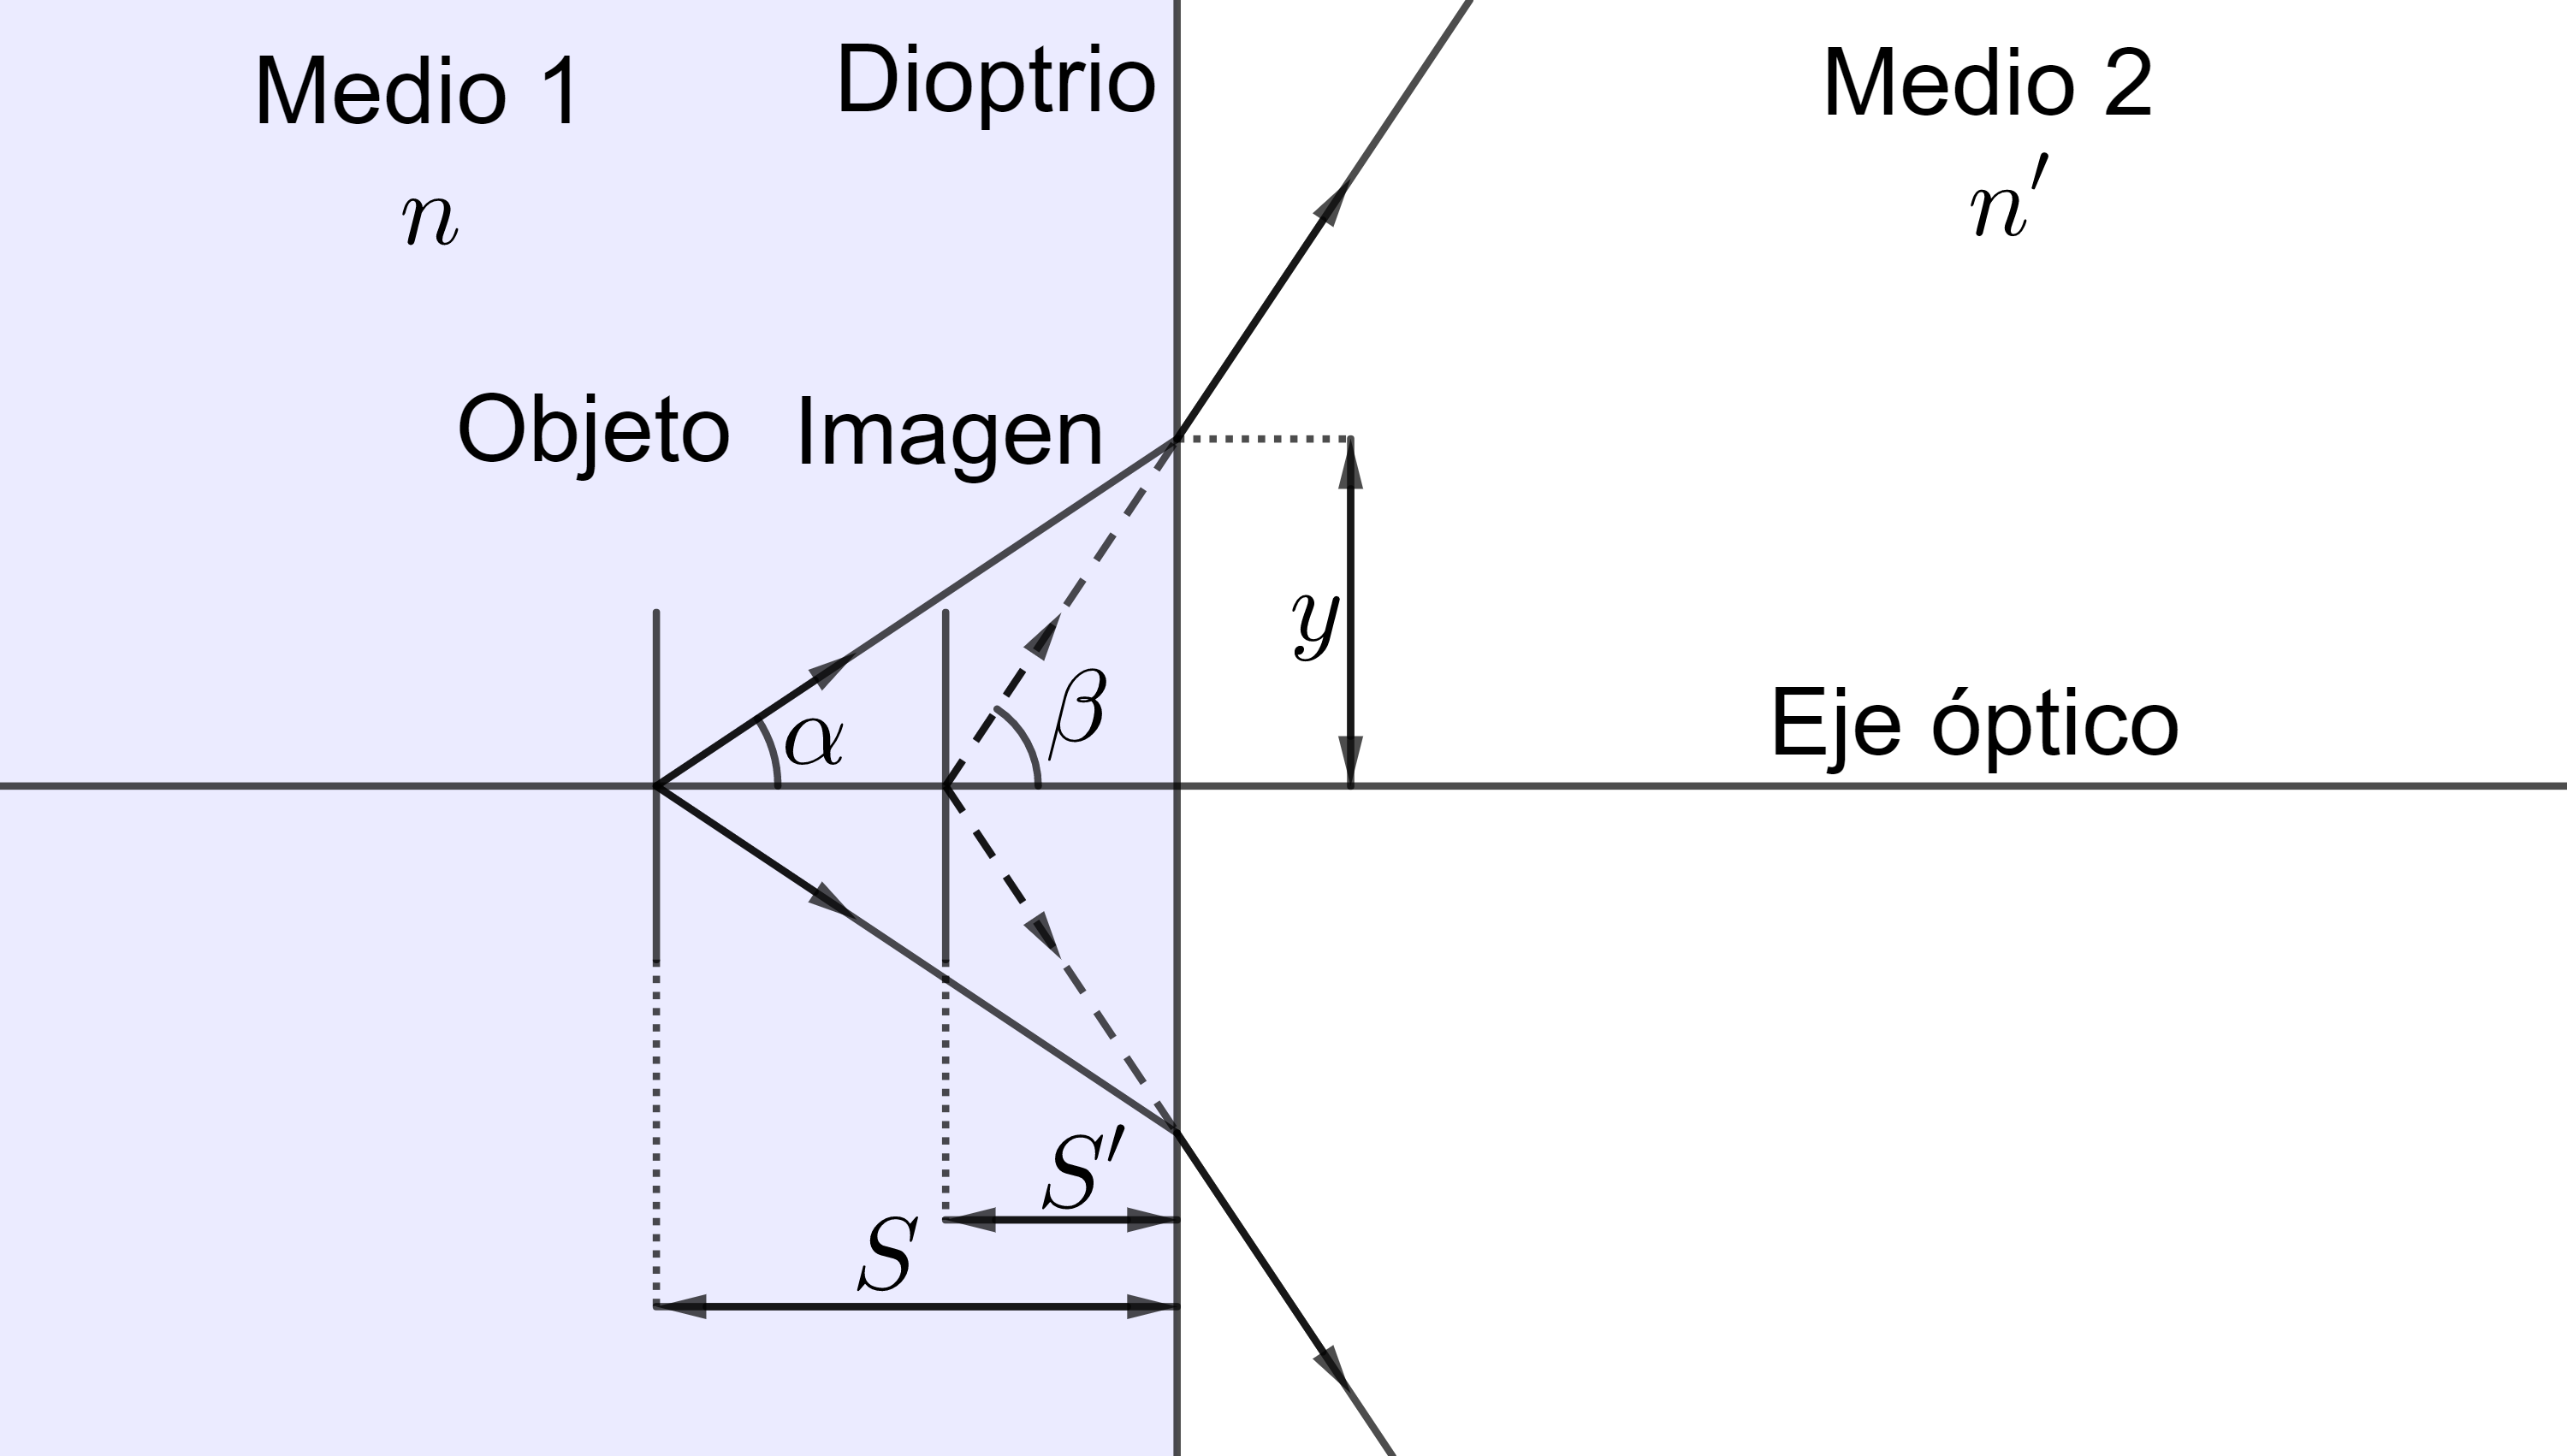
\includegraphics[width=10cm]{P2Refraccion.png}
\caption{Esquema de la imagen formada por refracción en un dioptrio plano.}
\label{P2refraccion}
\end{center}
\end{figure}

En la figura \ref{P2refraccion} se ve un esquema de lo que ocurre, donde $s$ es la distancia del objeto al dioptrio y $s'$ es la distancia de la imagen al dioptrio. La ley de Snell nos dice que $\frac{\sen\alpha}{\sen\beta}=\frac{n'}{n}$. Por trigonometría tenemos $\tan\alpha=\frac{y}{s}$ y $\tan\beta=\frac{y}{s'}$, que se resume en $\frac{\tan\alpha}{\tan\beta}=\frac{s'}{s}$. En el caso paraxial ---es decir, para rayos que forman un ángulo pequeño con el eje óptico--- los ángulos $\alpha$ y $\beta$ son muy pequeños se puede hacer la aproximación $\sen\alpha\approx\tan\alpha$ y $\sen\beta\approx\tan\alpha$, con lo que queda $\frac{n'}{n}=\frac{\sen\alpha}{\sen\beta}\approx\frac{\tan\alpha}{\tan\beta}=\frac{s'}{s}$.
\begin{equation}\label{P2distimagen}
s'=\frac{n'}{n}s
\end{equation} 

Sin embargo esta expresión es aproximada, pues según el ángulo con que sale un rayo del objeto, su imagen está en un sitio u otro como se ve en la figura \ref{P2astigmatismo}. Pero los rayos paraxiales forman la imagen todos ellos casi en el mismo sitio.

\begin{figure}[!ht]
\begin{center}
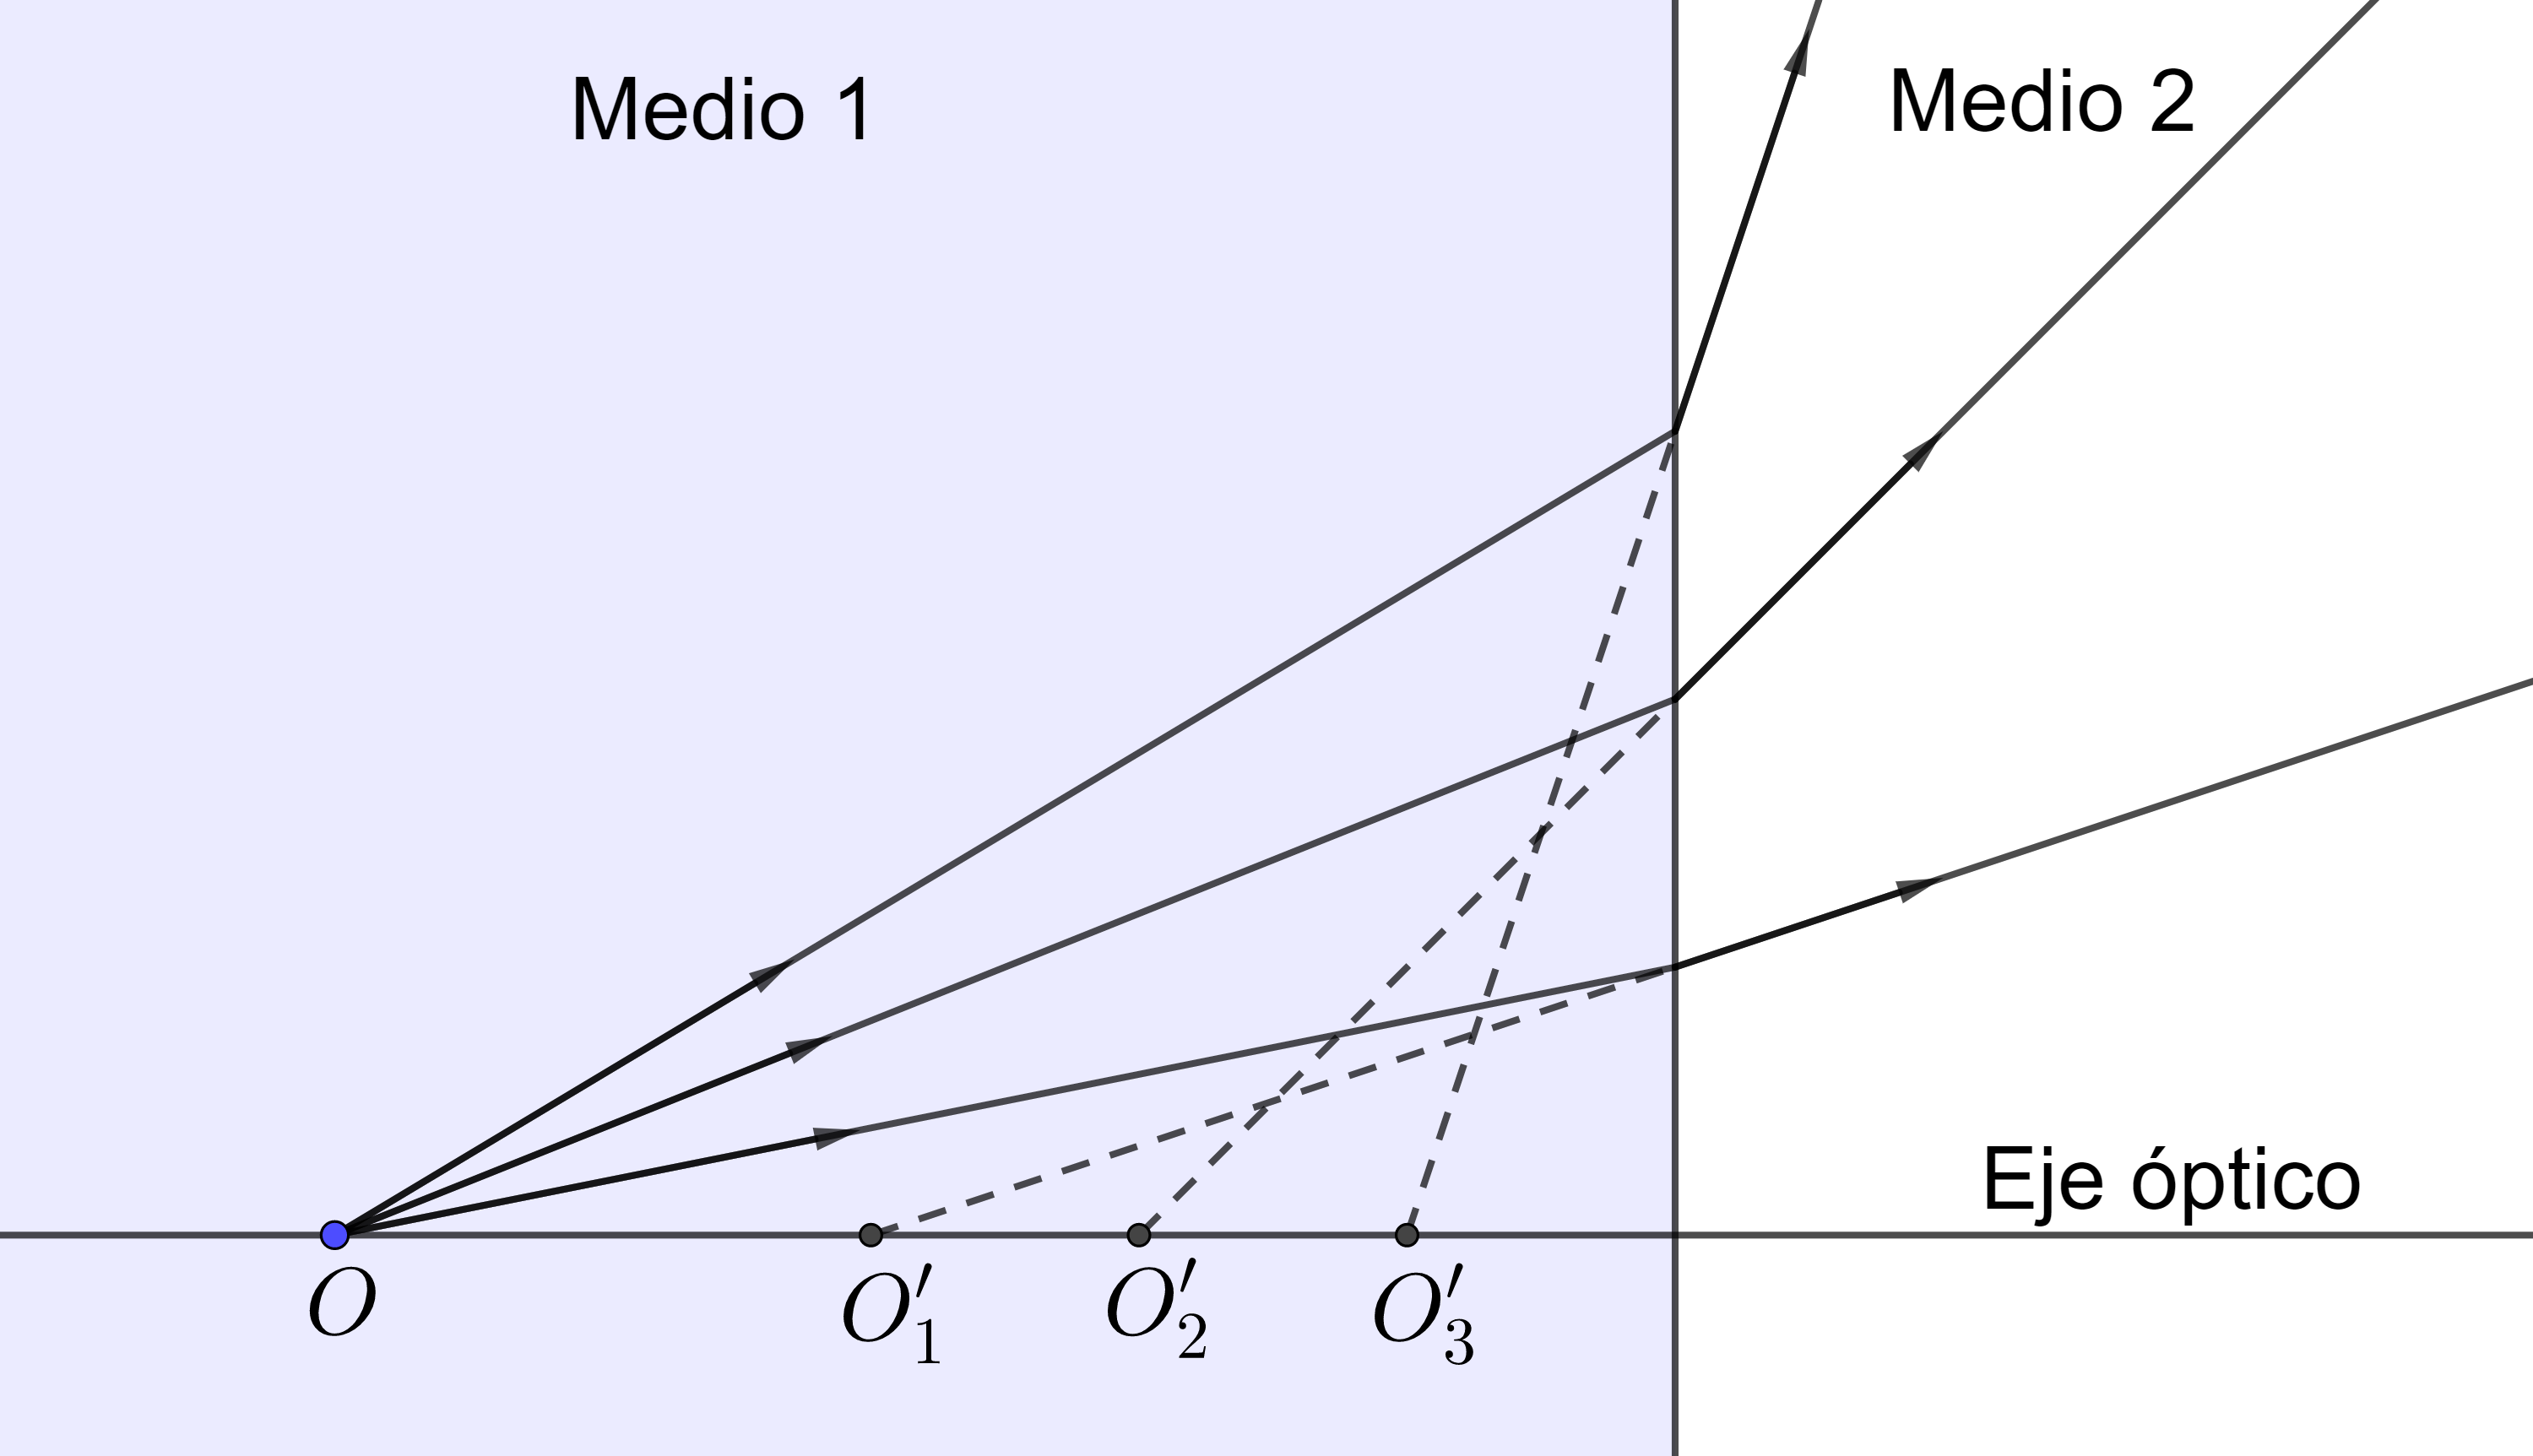
\includegraphics[width=10cm]{P2Astigmatismo.png}
\caption{Esquema de las distintas imágenes formadas por refracción en un dioptrio plano según el ángulo de inclinación de los rayos.}
\label{P2astigmatismo}
\end{center}
\end{figure}

Cuando se forma una imagen clara y nítida se dice que el dioptrio es estigmático.

Se quiere utilizar la ecuación (\ref{P2distimagen}) para calcular el índice de refracción de una lámina de vidrio. Para ello se pintan unas rayas en ambas caras de la lámina. Una de las rayas actuará de objeto y el grosor de la lámina será la distancia que separe el objeto del dioptrio $s$. Este dioptrio separa dos medios: vidrio y aire; por lo tanto, $n'$ será el índice de refracción del aire, el cual consideraremos, 0 y $n$ será el índice del vidrio.

El grosor de la lámina se mide con un comparador: se coloca la lámina en la platina y se miden las posiciones de la platina y de la parte superior de la lámina. Su diferencia será el grosor buscado. Se realizan varias medidas con el fin de disminuir la incertidumbre. La incertidumbre de cada medida directa es la precisión del comparador: $\unit[0.010]{mm}$. La de la diferencia es la anterior multiplicada por $\sqrt{2}$. El valor que se tomará es el de la media aritmética, con incertidumbre la raíz de la suma cuadrática de la incertidumbre experimental y la desviación típica de la media.

\begin{table}[!ht]
\caption{Tabla con las medidas de las posiciones de la platina y la lámina ---con incertidumbre $\unit[0.010]{mm}$--- junto a su diferencia ---con incertidumbre $\unit[0.014]{mm}$---, que es el grosor de la lámina. Todas las medidas están en milímetros.}
\label{P2tablaverdadero}
\begin{center}
\begin{tabular}{c|ccccc}
&Medida 1&Medida 2&Medida 3&Medida 4&Medida 5\\\hline
Posición 1&11,870&11,880&11,860&11,900&11,890\\
Posición 2&26,480&26,510&26,490&26,540&26,520\\\hline
Diferencia&14,610&14,630&14,630&14,640&14,630
\end{tabular}
\end{center}
\end{table}

En la tabla \ref{P2tablaverdadero} se encuentran estas medidas, de las que se deduce que el grosor medio de la placa es $s=\unit[(14.628\pm0.014)]{mm}$
\\

Ahora se mide la distancia de la imagen al dioptrio. Para ello se utiliza un microscopio y se calcula restando la posición de la platina a la que se enfoca el objeto visto a través del vidrio y la posición de la misma a la que se enfoca un dibujo pintado en la cara superior.

El microscopio tiene dos diafragmas: el diafragma de campo y el diafragma de apertura. El primero regula el área iluminada: el círculo iluminado será tanto mayor cuanto más abierto esté el diafragma y viceversa. Se sitúa en la parte inferior del microscopio. El segundo controla la inclinación de los rayos: al cerrarse el diafragma se dejan pasar únicamente los rayos más paraxiales.

Con el microscopio de que se dispone para esta práctica se comprueba que al abrir y cerrar el diafragma de la base del microscopio se amplía y se reduce el círculo iluminado en la muestra, lo que quiere decir que es el de campo.

Con el otro diafragma, el área iluminada se ve más iluminada o menos según se abre y se cierra. La muestra se ve igual de enfocada con este diafragma abierto o cerrado porque el desenfoque que produce que los rayos no sean del todo paraxiales no es muy grande. Sin embargo el que cambie cuánto está iluminado indica que se dejan pasar más rayos o menos, pues al limitar el paso a solo los rayos paraxiales; los que no lo son dejan de iluminar la muestra. Por lo tanto este diafragma es el de apertura.

Cuando los rayos que llegan al microscopio son paraxiales, se es capaz de conseguir un mejor enfoque, pues el sistema es estigmático y la imagen que se forma es muy nítida. Sin embargo existe una amplia región del espacio donde al colocar la muestra se ve bastante bien enfocada. Por su parte, cuando los rayos son oblicuos, el máximo enfoque posible no es tan bueno como el que se conseguiría con los rayos paraxiales y además la región del espacio en la que se puede enfocar medianamente bien está mucho más concentrada alrededor del plano focal.

No obstante, que los rayos no sean paraxiales será útil en esta práctica porque lo que interesa no es conseguir un enfoque perfecto, sino saber con precisión en qué punto se enfoca bien.

\begin{table}[!ht]
\caption{Tabla con las medidas de las posiciones aparentes de las caras superior e inferior de la lámina de vidrio ---con incertidumbre $\unit[0.010]{mm}$--- junto a su diferencia ---con incertidumbre $\unit[0.014]{mm}$---, que es el grosor aparente de la lámina. Todas las medidas están en milímetros. Las primeras medidas están hechas con el diafragma de apertura cerrado y después con el diafragma abierto.}
\label{P2tablaaparente}
\begin{center}
\begin{tabular}{c|c|ccccc}
\multicolumn{2}{c|}{}&Medida 1&Medida 2&Medida 3&Medida 4&Medida 5\\\hline
\multirow{3}{*}{Cerrado}&Posición 1&16,260&16,030&16,400&15,970&15,120\\
&Posición 2&25,980&25,620&25,700&25,660&25,650\\\cline{2-7}
&Diferencia&9,720&9,590&9,300&9,690&10,530\\\hline
\multirow{3}{*}{Abierto}&Posición 1&16,260&16,050&16,100&15,990&16,150\\
&Posición 2&25,700&25,580&25,680&25,730&25,820\\\cline{2-7}
&Diferencia&9,440&9,530&9,580&9,740&9,670
\end{tabular}
\end{center}
\end{table}

En la tabla \ref{P2tablaaparente} se encuentran las medidas del grosor aparente de la placa con el diafragma de apertura abierto y cerrado. La media del grosor con el diafragma cerrado es $\unit[(9.766\pm0.044)]{mm}$ y con el diafragma abierto es $\unit[(9.592\pm0.014)]{mm}$. Se puede apreciar que la incertidumbre con el diafragma abierto es aproximadamente tres veces menor que con el diafragma cerrado. Esta diferencia es más acusada si se observan las desviaciones típicas de las medias ---debidas únicamente a la dispersión de las medidas, sin tener en cuenta la precisión del aparato de medida---. La desviación típica con el diafragma cerrado es $\unit[0.042]{mm}$ y abierto es $\unit[0.0028]{mm}$, unas 15 veces menor.

Esto confirma lo que se había dicho antes: cuando se abre el diafragma la región donde el objeto se ve enfocado se reduce y por lo tanto las medidas se concentran más alrededor de la media.
\\

El índice de refracción de un material depende de la longitud de onda, produciéndose una dispersión cromática. Para comprobar esta dependencia en la lámina de vidrio, se verá cómo varían las medidas en función de la longitud de onda de la luz utilizada. Para ello se colocará un filtro que transmite la luz roja y un filtro que transmite la luz azul, dos colores con longitudes de onda lo más dispares posible dentro del rango visible.

Se ha visto que con el diafragma de apertura abierto se obtienen unos resultados más precisos, de modo que para esta parte de la práctica se deja el diafragma abierto.

\begin{table}[!ht]
\caption{Tabla con las medidas de las posiciones aparentes de las caras superior e inferior de la lámina de vidrio ---con incertidumbre $\unit[0.010]{mm}$--- junto a su diferencia ---con incertidumbre $\unit[0.014]{mm}$---, que es el grosor aparente de la lámina. Todas las medidas están en milímetros. Las primeras medidas están hechas con un filtro rojo y después con un filtro azul.}
\label{P2tablacolores}
\begin{center}
\begin{tabular}{c|c|ccc}
\multicolumn{2}{c|}{}&Medida 1&Medida 2&Medida 3\\\hline
\multirow{3}{*}{Rojo}&Posición 1&15,680&15,510&15,580\\
&Posición 2&25,200&25,080&25,260\\\cline{2-5}
&Diferencia&9,520&9,570&9,680\\\hline
\multirow{3}{*}{Azul}&Posición 1&15,650&15,510&15,570\\
&Posición 2&25,090&24,950&25,180\\\cline{2-5}
&Diferencia&9,440&9,440&9,610
\end{tabular}
\end{center}
\end{table}

La media del grosor con el filtro rojo es $\unit[(9.590\pm0.014)]{mm}$ y con el azul es $\unit[(9.497\pm0.015)]{mm}$. Vemos que no son compatibles, lo que quiere decir que se pueden considerar distintas. La dispersión cromática en esta lámina de vidrio no es despreciable.

Finalmente se calcula el índice de refracción de la lámina de vidrio usada en esta práctica gracias a la fórmula (\ref{P2distimagen}). Su incertidumbre es calculada mediante la fórmula de propagación de incertidumbres. Sin poner ningún filtro con el diafragma abierto el índice calculado es $1.5250\pm0.0027$. El índice de refracción para la longitud de onda del rojo vale $1.5253\pm0.0027$ y para el azul $1.5403\pm0.0028$. Efectivamente el índice de refracción es distinto para cada longitud de onda. Cuando no se pone ningún filtro el índice de refracción es muy parecido al del rojo. Esto ocurre porque el objeto que se ha usado era de color rojo, de modo que la luz proveniente del objeto era mayoritariamente roja.

Con el diafragma cerrado se tiene un índice de refracción igual a $1.4978\pm0.0069$, que dista mucho de los tres valores anteriores por las razones ya explicadas.

\subsection{Efecto Pffund}

Cuando se hace incidir un rayo de luz sobre una superficie y se refleja, puede salir reflejado de dos formas principalmente: especular y difusa. La primera se produce cuando la superficie es pulida y sale formando el mismo ángulo con la normal. La segunda ocurre cuando la superficie es rugosa.

En realidad la reflexión es siempre especular, pero cuando la superficie es rugosa, en cada punto la normal puede tener cualquier inclinación y por lo tanto al final el rayo puede ser reflejado en cualquier dirección.
\\

Para esta práctica se utiliza un láser. Primero se observarán una serie de cosas para entender mejor la propagación rectilínea de la luz y la reflexión especular y difusa.

El láser se dispone para que su luz salga horizontal. Se utiliza un espejo a $\unit[45]{º}$ para hacer que el haz caiga perpendicular sobre la mesa. Entre el espejo y la mesa se pone una lente que focaliza la luz. Al encender el láser, el rayo de luz no se ve, pues solo se ven los puntos desde los que sale un rayo que llega al ojo. Se ve principalmente el punto de la mesa al que llega el haz de luz y se refleja difusamente. Sin embargo también se ven puntos muy débiles en el espejo y en la lente que no deberían verse, pero hay una fracción mínima de la luz que se refleja de forma difusa y acaba llegando al ojo.

Ahora se apunta con el láser al espejo por la cara de aluminio. Esta cara es pulida y opaca, por lo que toda la luz que incide es reflejada de forma especular. Al apuntar, sin embargo, se ve un punto rojo muy débil. Como antes, una pequeña parte del rayo es reflejado difusamente y llega al ojo.

Cuando se apunta con el láser al papel satinado una parte se refleja y otra parte se refracta a partes quizá no iguales, pero sí similares. El papel es rugoso, así pues la reflexión y la transmisión son difusas, es decir, el rayo sale en todas las direcciones. Gracias a esto en cualquier posición el rayo llega al ojo y se ve un punto rojo en el punto donde incide el láser. Cuando se mira el papel por el lado en el que está el láser, la luz llega al ojo por reflexión. Cuando se mira por el lado donde no está el láser, el rayo llega al ojo refractándose en el papel.

Con el plástico blanco, como es opaco, la luz no lo atraviesa: no se refracta. Solo se refleja y lo hace de forma especular. Cuando se mira detrás del plástico no se ve nada y si se mira la cara enfrentada al aparato láser, se ve un punto rojo fruto de la reflexión difusa.
\\

Se dispone de un espejo óptico que en un lado tiene aluminio pulido y opaco que refleja la luz de modo especular. El otro lado es de un vidrio que transmite la luz. Cuando el haz incide sobre la cara vítrea, una parte es reflejada y otra es transmitida al interior. Al llegar a la cara de aluminio se refleja y después llega otra vez a la superficie vidrio-aire y parte es transferida al exterior y otra parte se queda reflejada en el interior. Cada vez que se refleja la luz en la cara de vidrio, pierde intensidad porque parte de la luz se está transmitiendo. Se puede ver un esquema de lo que ocurre en la figura \ref{P2espejo}.

\begin{figure}[!ht]
\begin{center}
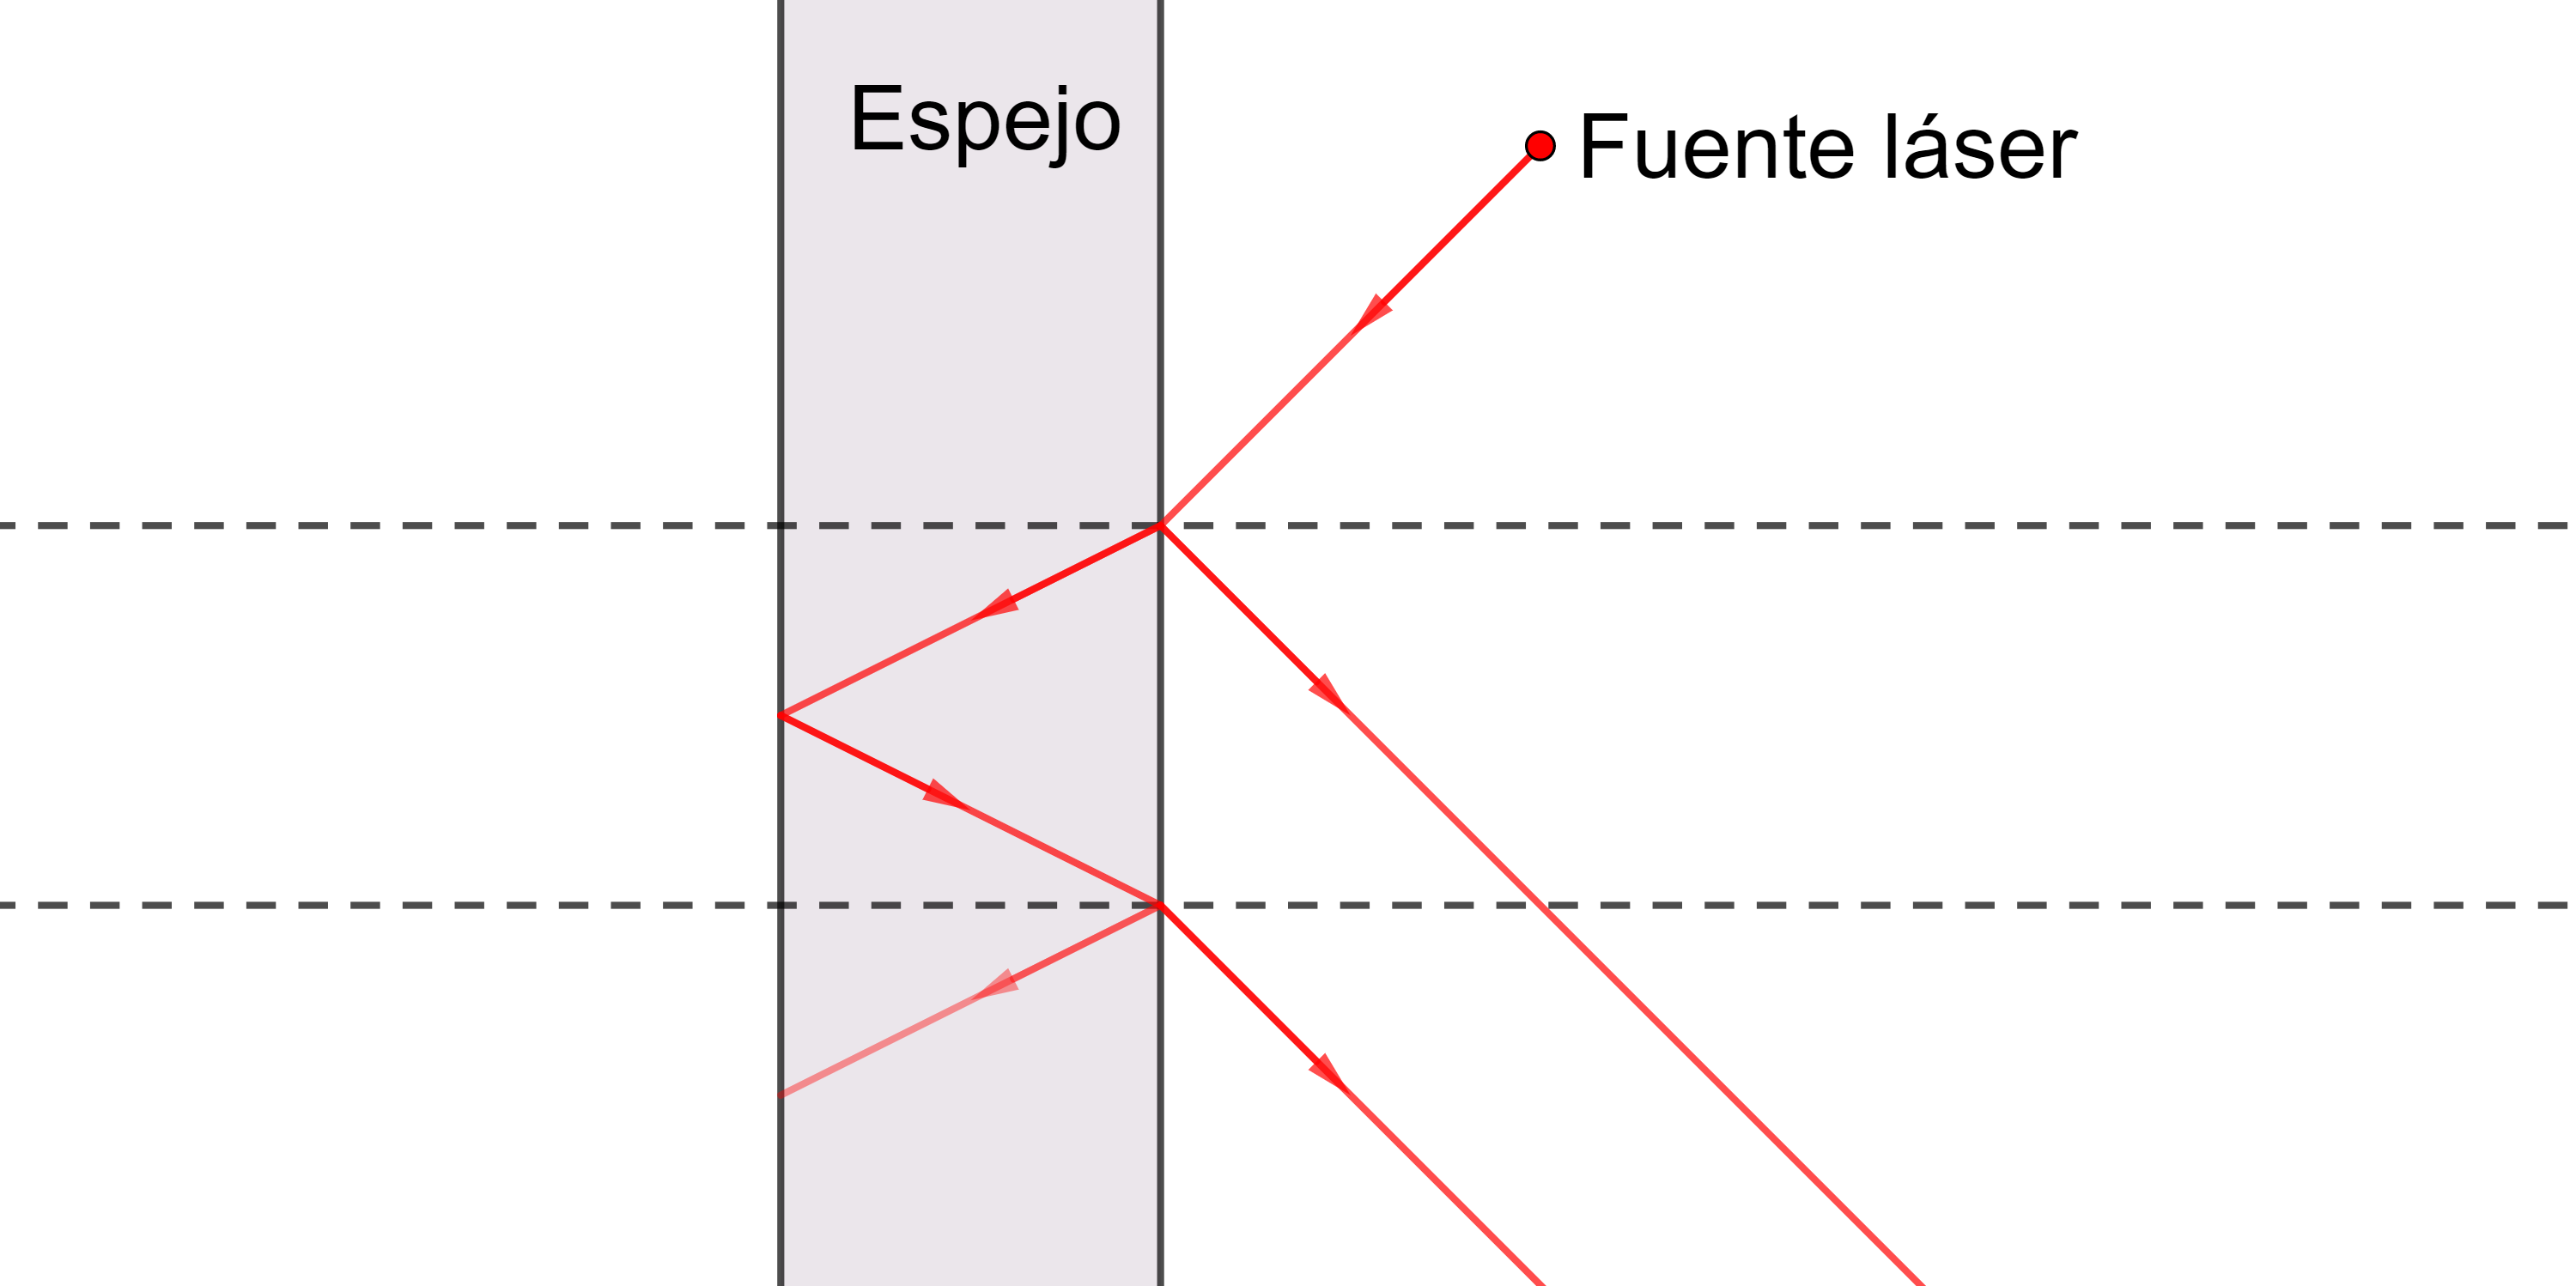
\includegraphics[width=8cm]{P2Espejo.png}
\caption{Esquema de un haz de luz láser que entra a un espejo con una cara izquierda opaca y con el resto de vidrio.}
\label{P2espejo}
\end{center}
\end{figure}

Cuando se proyecta la luz del láser sobre el espejo se observan un punto intenso y cinco puntos a su alrededor más débiles. El punto central es el rayo procedente del laser que se refracta en la cara de vidrio, se refleja en la cara de aluminio y luego se vuelve a refractar saliendo al exterior. Los otros son resultado del rayo anterior que, en su última refracción, en lugar de salir al aire, se refleja otra vez, va hasta la cara opaca del espejo, se refleja y al final se refracta en la cara del vidrio y sale. Estos últimos puntos son más débiles por la pérdida de intensidad comentada en el parágrafo anterior.

Al inclinar el espejo los puntos se ven más brillantes porque cuando los rayos llegan a la superficie vidrio-aire desde la parte del vidrio lo hacen con un ángulo de incidencia mayor, más próximo al ángulo límite. Por lo tanto se refleja más luz que antes y llega más luz a los puntos que rodean el punto central. Por esto se ven más brillantes.
\\

Por la ley de Snell si un rayo de luz llega a una superficie de separación entre dos medios con índices de refracción $n$ y $n'$ y forma un ángulo $\varepsilon$ con la recta normal a la superficie, el rayo saldrá desviado formando un ángulo $\varepsilon'$ con la normal.
\begin{equation}\label{P2Snell}
\frac{\sen\varepsilon'}{\sen\varepsilon}=\frac{n}{n'}
\end{equation}
Otra forma de escribir (\ref{P2Snell}) es $\sen\varepsilon'=\frac{n}{n'}\sen\varepsilon$. Si $n>n'$, existirá un ángulo de incidencia $\varepsilon$ tal que el rayo refracto forme un ángulo $\varepsilon'=\unit[\frac{\pi}{2}]{rad}$. Este ángulo se conoce como ángulo límite $\varepsilon_l$. En este caso $\sen\varepsilon'=1$.
\begin{equation}\label{P2eqangulolimite}
\sen\varepsilon_l=\frac{n'}{n}
\end{equation}
Este ángulo existe porque por hipótesis $\frac{n'}{n}<1$. Si el ángulo de incidencia es mayor que el ángulo límite $\epsilon>\epsilon_l$, entonces $\sen\varepsilon>\sen\varepsilon_l$ y $\sen\varepsilon'=\frac{n}{n'}\sen\varepsilon>\frac{n}{n'}\sen\varepsilon_l>\frac{n}{n'}\frac{n'}{n}=1$. Sin embargo no existe ningún ángulo real cuyo seno sea mayor que 1. Por lo tanto si el ángulo de incidencia es mayor que el ángulo límite, no existirá un rayo transmitido: todo el rayo será reflejado. Este fenómeno se conoce como reflexión total y se puede ver un esquema en la figura \ref{P2figangulolimite}.

\begin{figure}[!ht]
\begin{center}
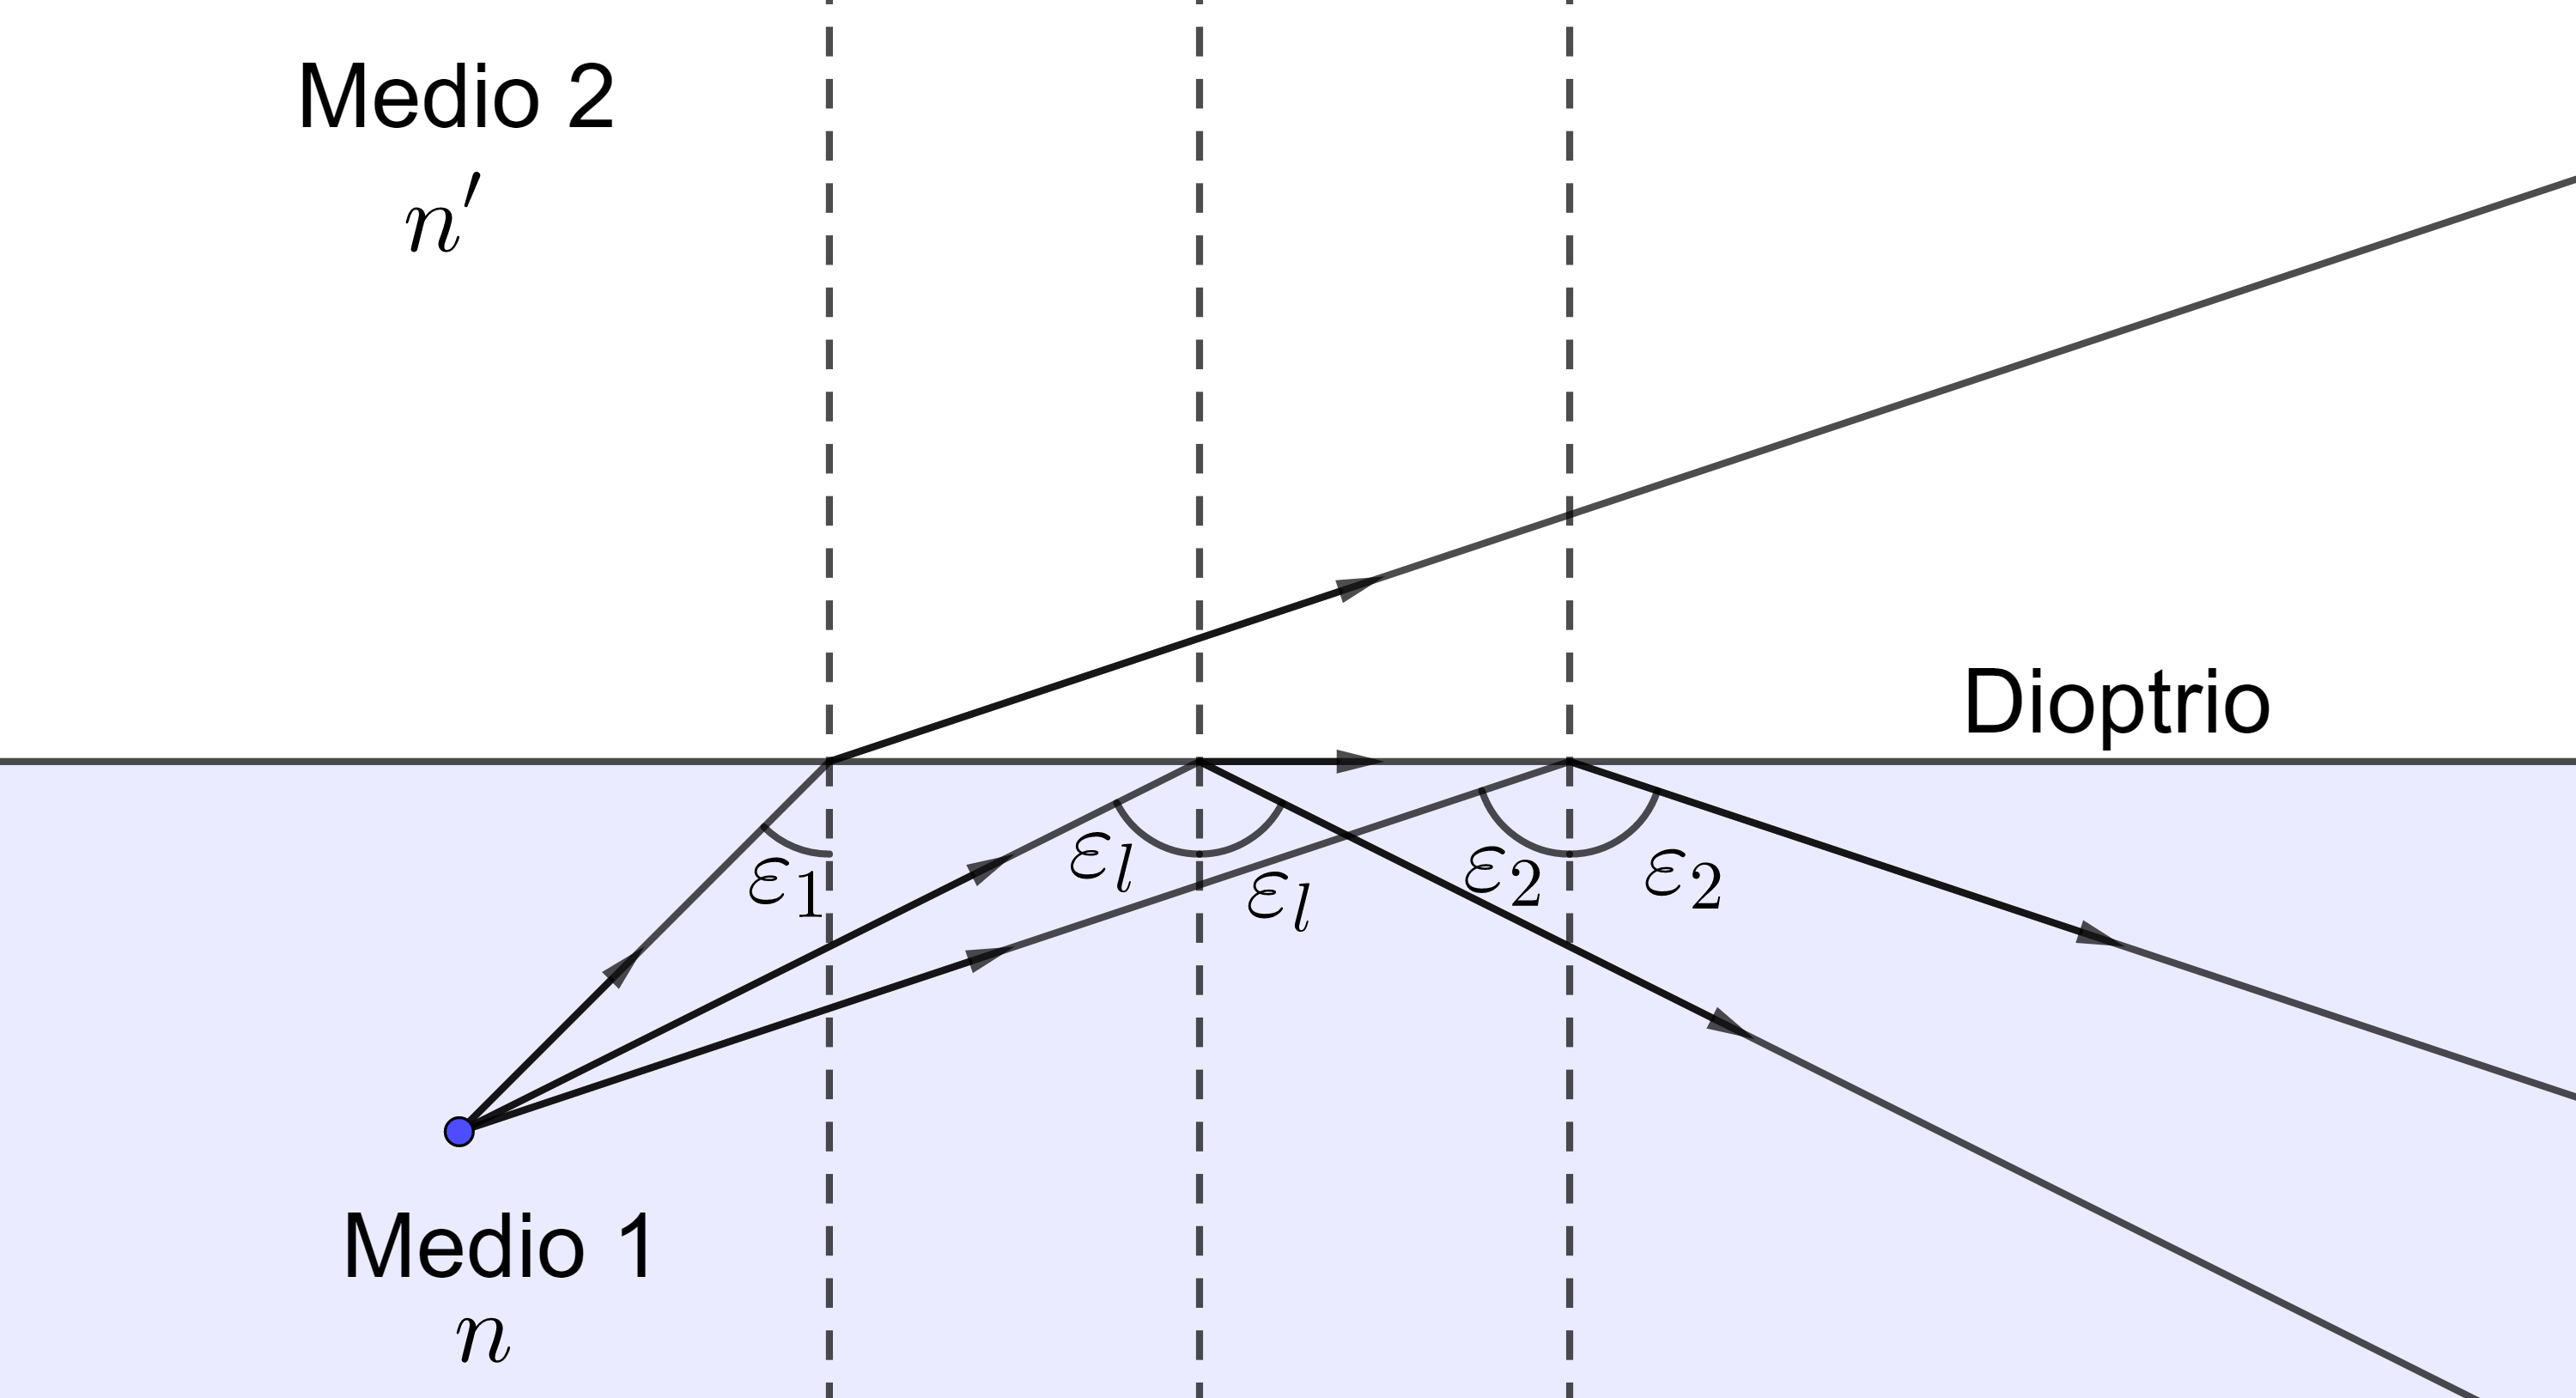
\includegraphics[width=10cm]{P2Angulolimite.png}
\caption{Esquema de la reflexión y refracción de rayos con distinto ángulo de incidencia. Cuando este supera el ángulo límite, el rayo es reflejado íntegramente.}
\label{P2figangulolimite}
\end{center}
\end{figure}

Siempre que un rayo de luz llega a un dioptrio, una fracción es refractada y la fracción complementaria es reflejada. Cuando $n>n'$, conforme aumenta el ángulo de incidencia, la fracción refractada se va haciendo cada vez más pequeña en favor de la reflejada. Hasta que se llega al ángulo límite, a partir del cual todo el rayo es reflejado.
\\

El concepto de reflexión total es en el que se basa el efecto Pffund.

Se vierte agua sobre la mesa y se forma una fina lámina plana de agua. La luz del láser cae verticalmente sobre el agua y llega a la mesa en el punto $A$ de la figura \ref{P2PffAgua}. Ahí se refleja de forma difusa en todas las direcciones, entre ellas la que llega al ojo. Ese punto se ve iluminado. De ahí los rayos que salen poco inclinados llegan a la superficie y se refractan casi enteramente y muy poca parte del rayo se refleja. El rayo que sale del punto $A$ con un ángulo de inclinación igual al ángulo límite, ---el cual existe porque el índice del agua es mayor que el del aire---, llega al punto $B$ y se refleja íntegro de forma especular llegando al punto $C$, donde se refleja de forma difusa y este punto se ve iluminado. Los rayos que tienen una inclinación mayor que el ángulo límite también se reflejan íntegros y llegan a la mesa más allá del punto $C$.

\begin{figure}[!ht]
\begin{center}
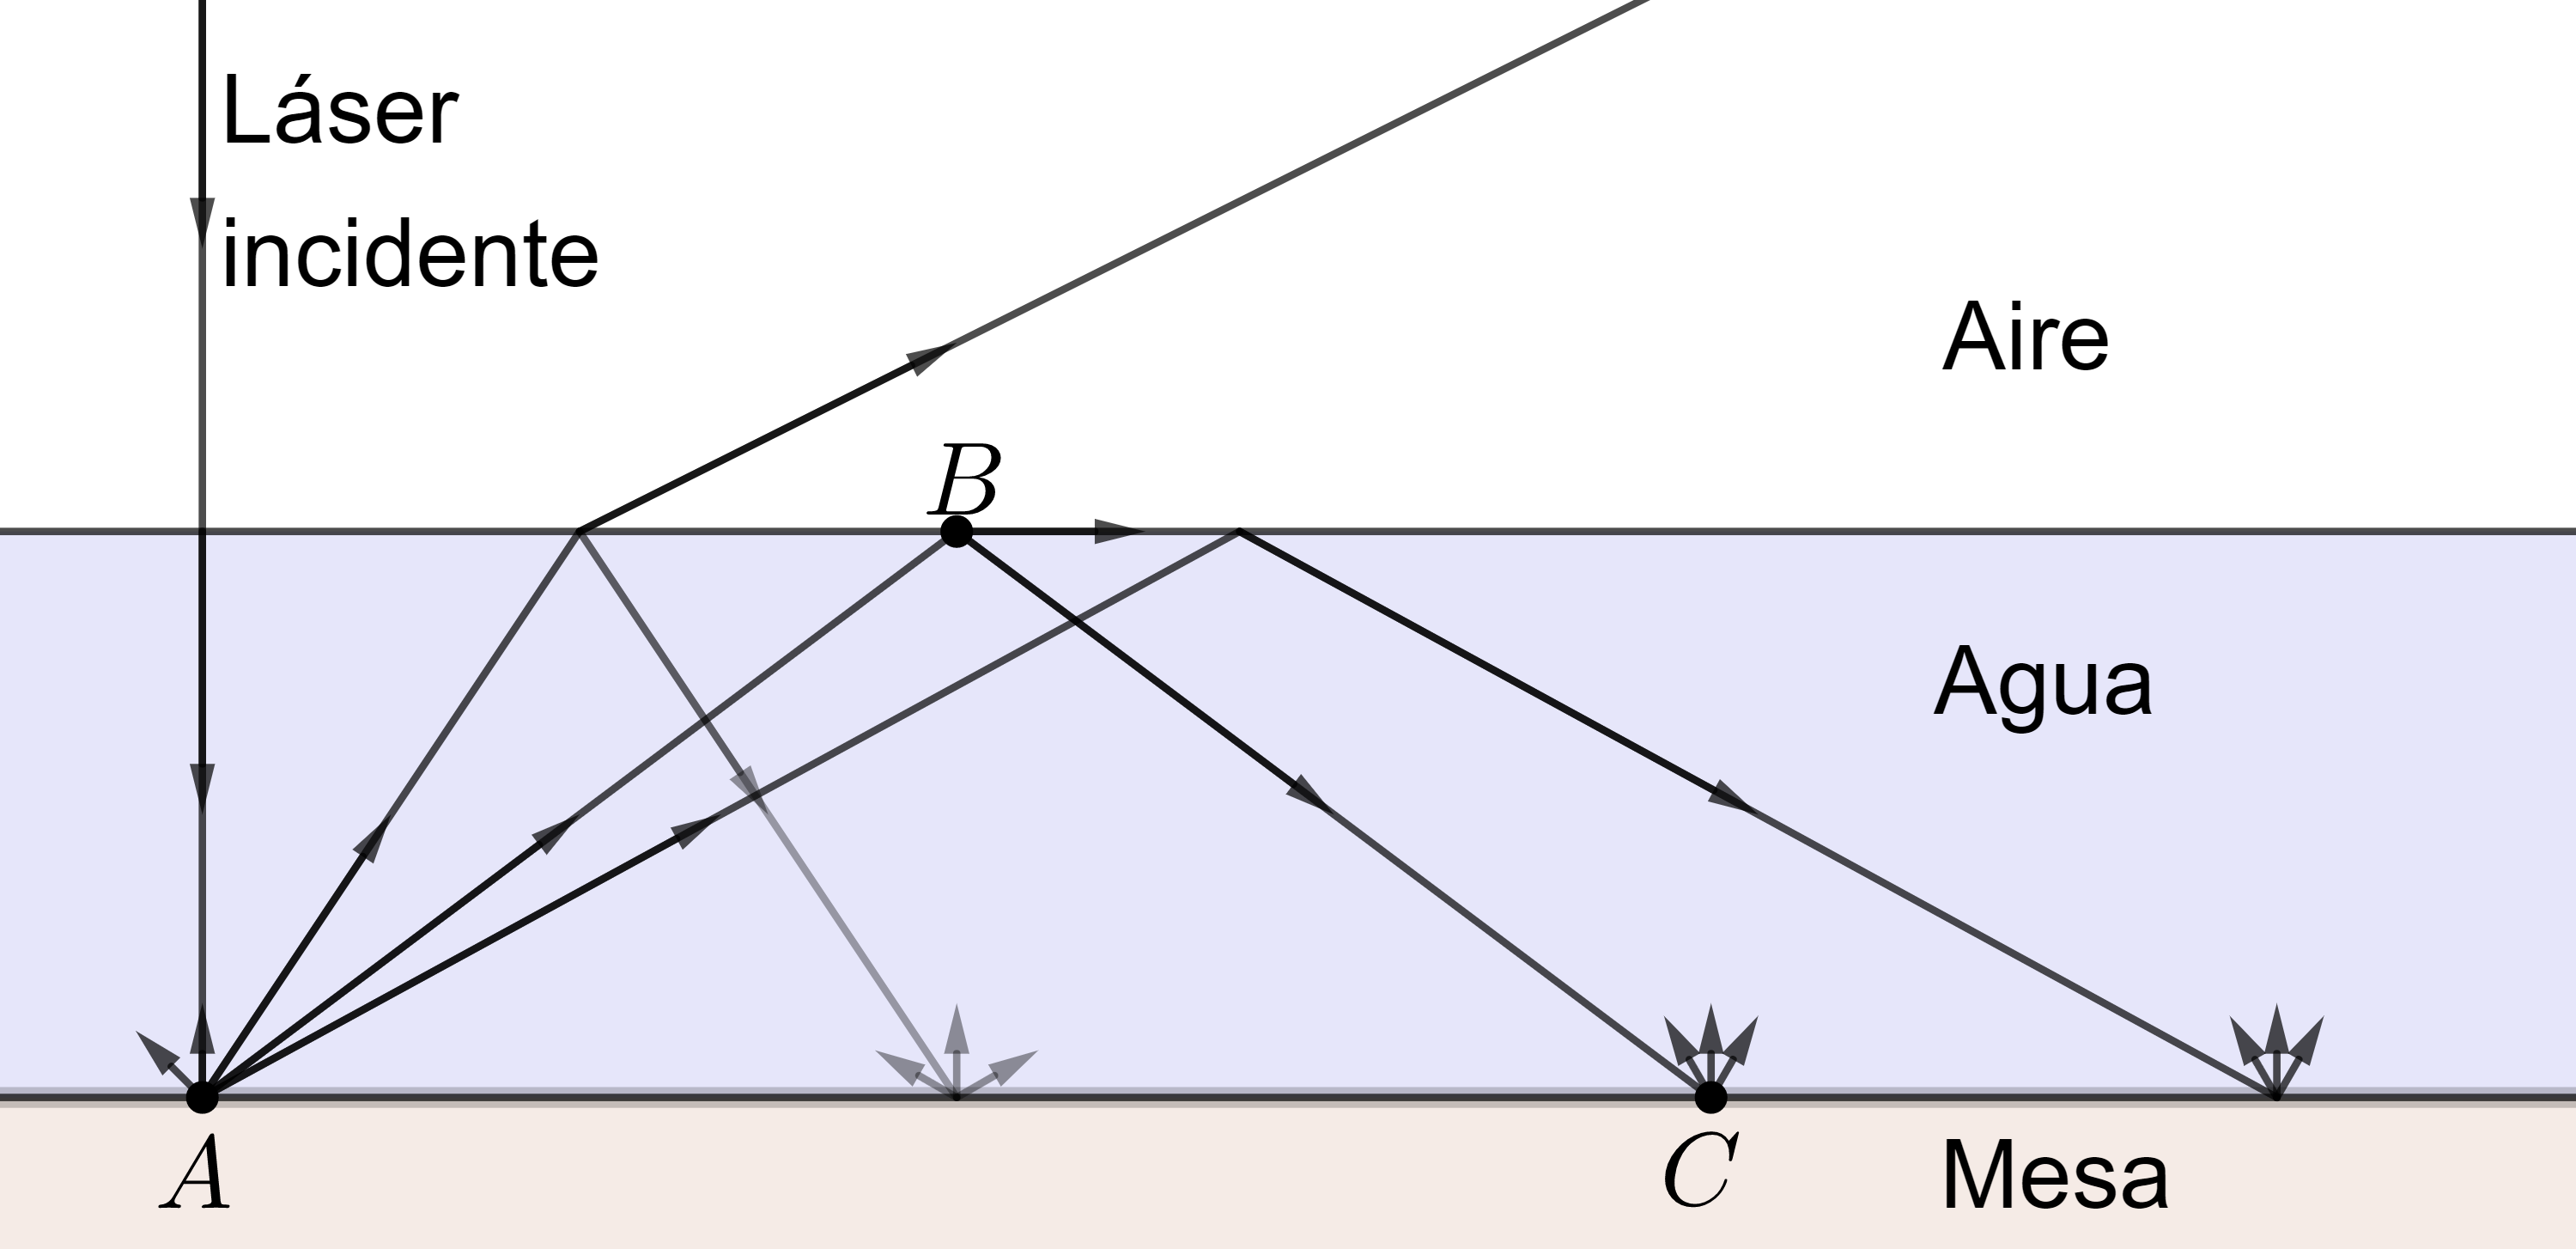
\includegraphics[width=10cm]{P2PffAgua.png}
\caption{Esquema del efecto Pffund sobre una lámina de agua.}
\label{P2PffAgua}
\end{center}
\end{figure}

El rayo que llega a $B$ lo hace con un ángulo de incidencia igual al ángulo límite $\sen\varepsilon_l=\frac{1}{n}$ donde $n$ es el índice de refracción del agua (el del aire se considera 1). Si la distancia entre los puntos $A$ y $C$ es $r$, la distancia horizontal entre $A$ y $B$ es $\frac{r}{2}$. Si $d$ es el grosor de la lámina de agua, tenemos $\tan\varepsilon_l=\frac{r}{2d}$. Así pues el radio de la zona oscura es $r=2d\tan\varepsilon_l$ donde $\sen\varepsilon_l=\frac{1}{n}$.

\begin{equation}\label{P2PffRadioParvo}
r=\frac{2d}{\sqrt{n^2-1}};\hspace{2mm}n=\sqrt{1+\frac{16d^2}{\phi^2}},\text{ donde }\phi=2r
\end{equation}

En resumen, en la gota se ve muy iluminado el punto $A$ sobre el que incide directamente el haz láser. Desde ese punto hasta el punto $C$ se ve una zona oscura y desde el punto $C$ hasta fuera de la gota se ve iluminado, aunque con menor intensidad, pues parte se ha perdido ya en la reflexión difusa del punto $A$. 

\begin{figure}[!ht]
\begin{center}
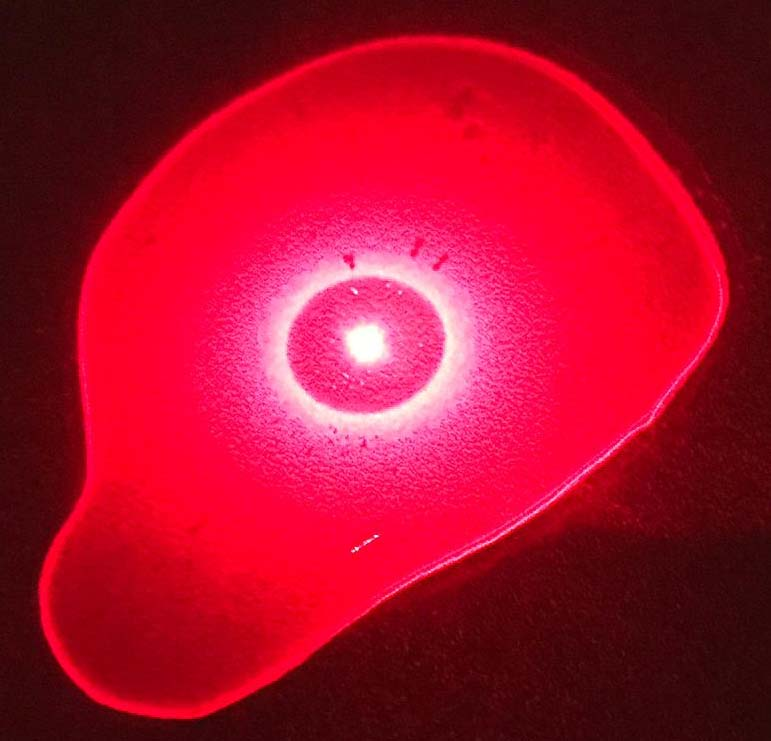
\includegraphics[width=7cm]{P2PffAgua.jpeg}
\caption{Fotografía de una superficie de agua sobre la mesa iluminada con un rayo láser ilustrando el efecto Pffund.}
\label{P2PffFotoAgua}
\end{center}
\end{figure}

La figura \ref{P2PffFotoAgua} es una fotografía que se hizo de este fenómeno. Se ve claramente un pequeño círculo brillante en el centro, luego una corona oscura y más allá otra corona brillante, lo cual concuerda con lo que se ha explicado de forma teórica.
\\

Ahora en lugar de una lámina de agua se pone una lámina de vidrio. Entre el vidrio y la mesa se forma una fina película de aire que cambia por completo lo que se observa. La figura \ref{P2PffVidrio} muestra un esquema de lo que les ocurre a los rayos. Sobre el punto $A$ se hace incidir el haz y de ahí se propaga en todas las direcciones. Los rayos que llegan a la cara superior de la lámina con un ángulo menor que el ángulo límite son en parte refractados y en parte reflejados. Su reflejo llega a la mesa y la ilumina. Sin embargo los rayos que llegan a la cara superior con un ángulo de incidencia igual ---o mayor--- al ángulo límite, son enteramente reflejados hacia abajo. Cuando llegan a la cara inferior de la lámina vuelven a llegar a una superficie de separación entre vidrio y aire. Por la ley de la refracción, al reflejarse el rayo en la cara superior sale con el mismo ángulo que el de incidencia, de modo que en la inferior el ángulo de incidencia es nuevamente el ángulo límite y el rayo se vuelve a reflejar totalmente. Así sucesivamente, dando lugar a una zona oscura.

Cuando se pone papel satinado en medio del camino del haz de luz, se dejan de ver los círculos y se pasa a ver una iluminación uniforme. Esto ocurre porque la luz atraviesa el papel, pero sale dispersa en todas las direcciones, mientras que sin el papel el haz de luz cae vertical.

\begin{figure}[!ht]
\begin{center}
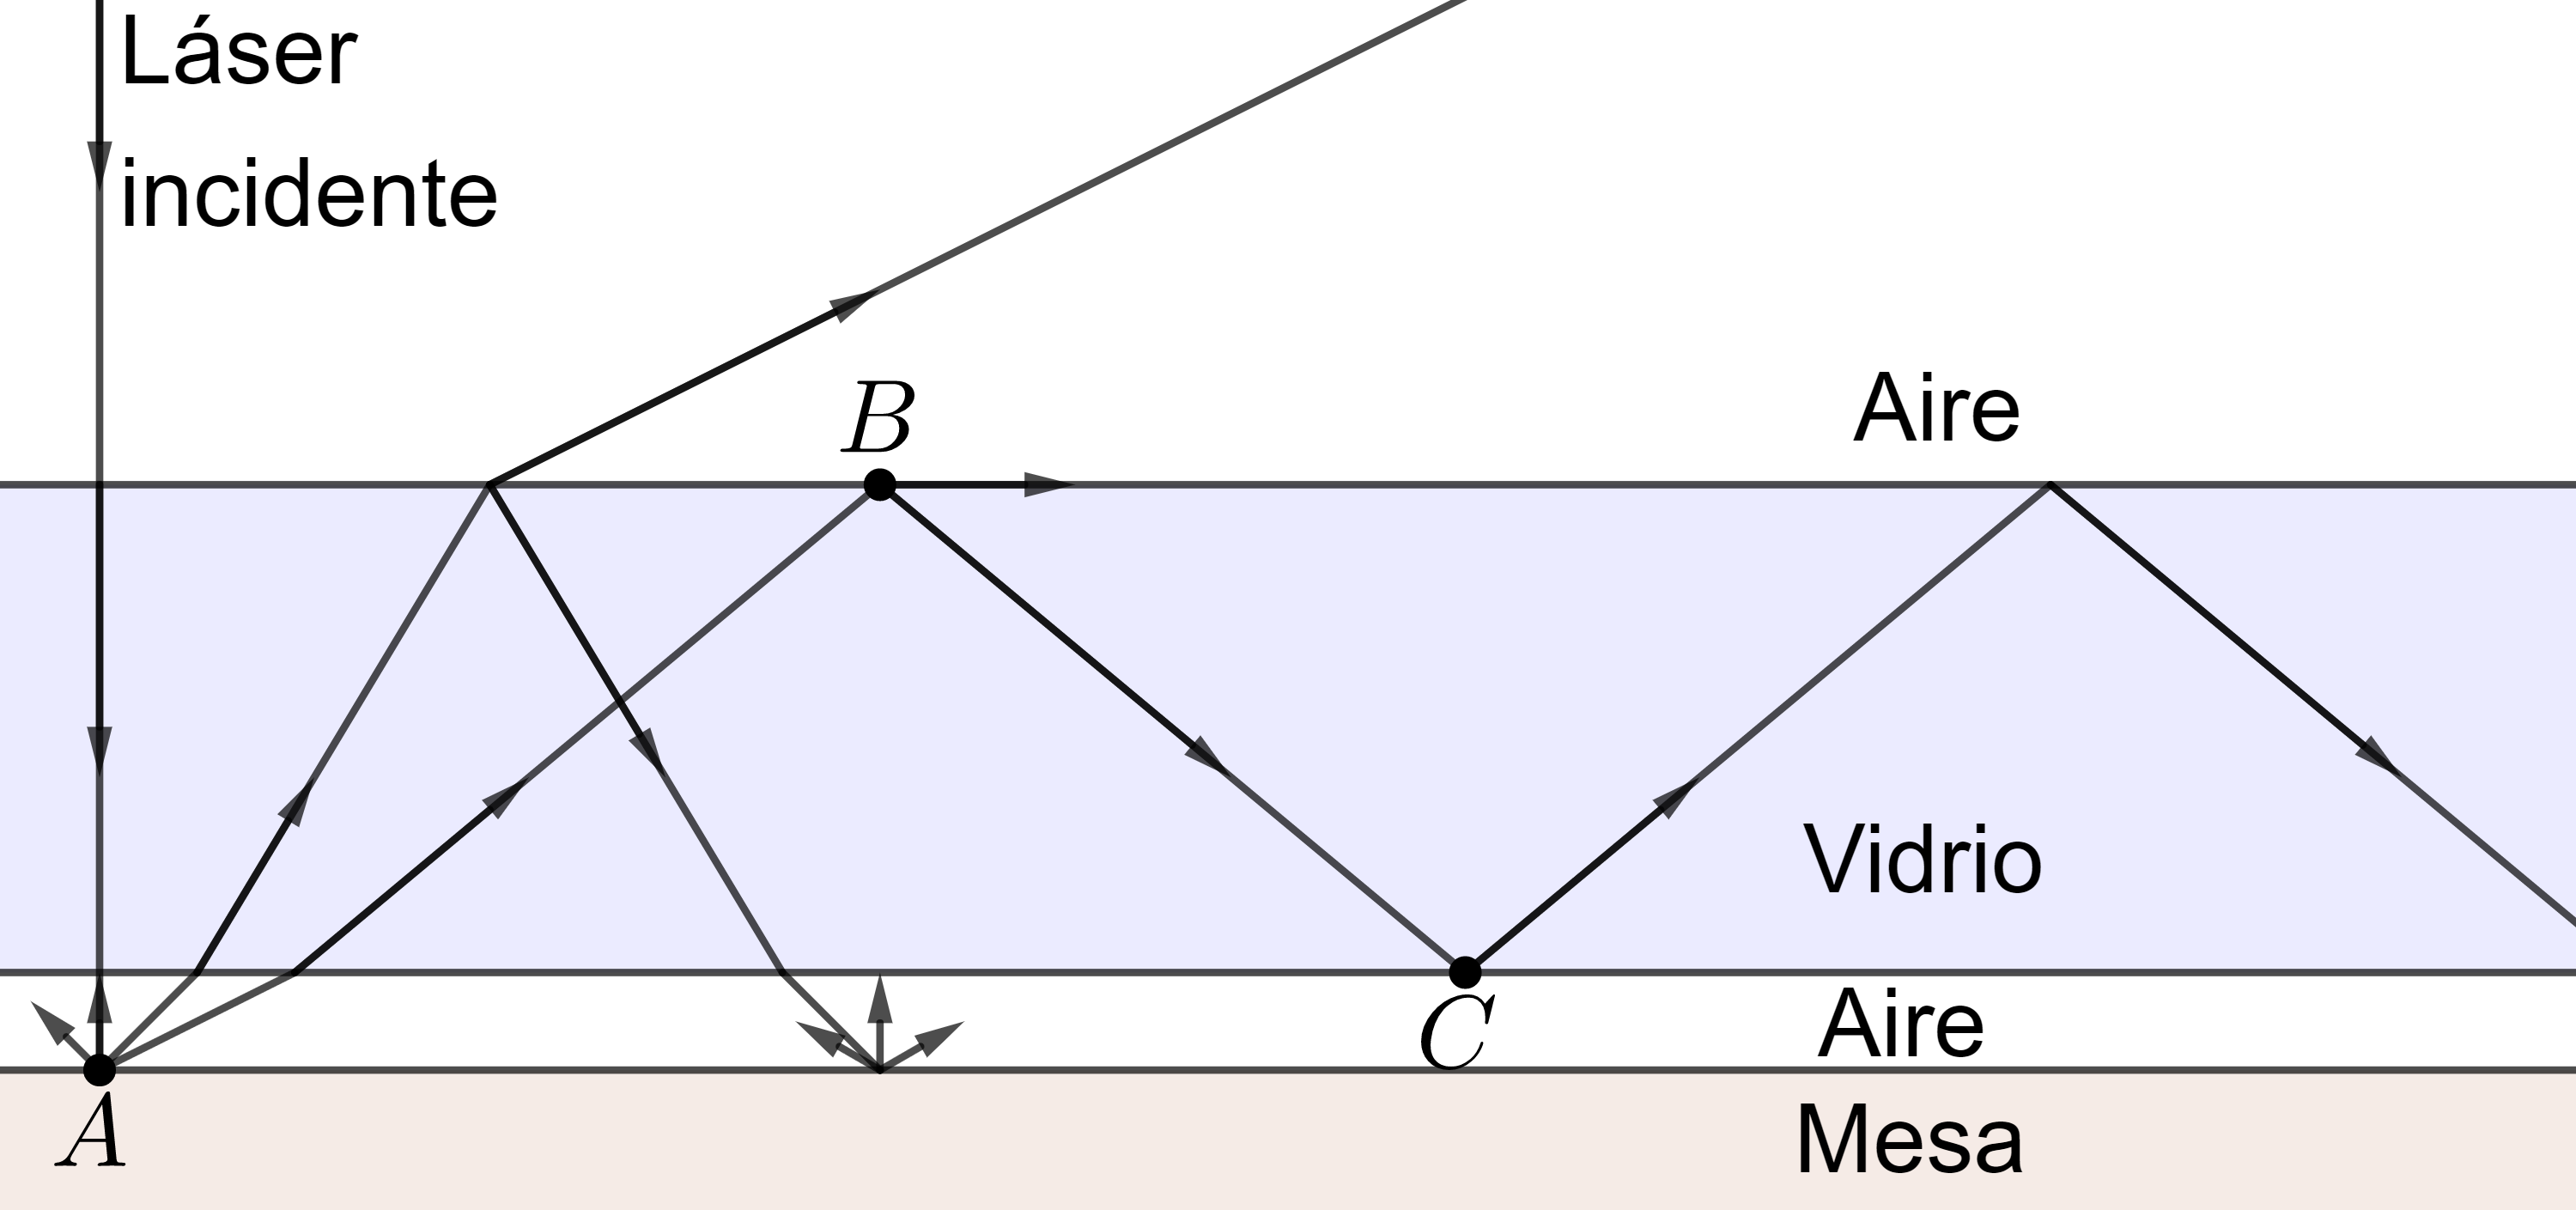
\includegraphics[width=10cm]{P2PffVidrio.png}
\caption{Esquema del efecto Pffund sobre una lámina de vidrio.}
\label{P2PffVidrio}
\end{center}
\end{figure}

Por lo tanto se debería observar un punto central muy iluminado, una corona a su alrededor menos iluminada y más allá de la corona se vería oscuro. Como la capa de aire tiene un grosor despreciable, el radio de la zona iluminada viene dado por la misma ecuación (\ref{P2PffRadioParvo}) que en el caso anterior cambiando el índice de refracción del agua por el del vidrio ($n$) y el grosor de la capa de agua por el de la lámina de vidrio ($d$). Esto se ve claramente en la fotografía izquierda de la figura \ref{P2PffFotoVidrio} obtenida experimentalmente.

\begin{figure}[!ht]
\begin{center}
\subfigure{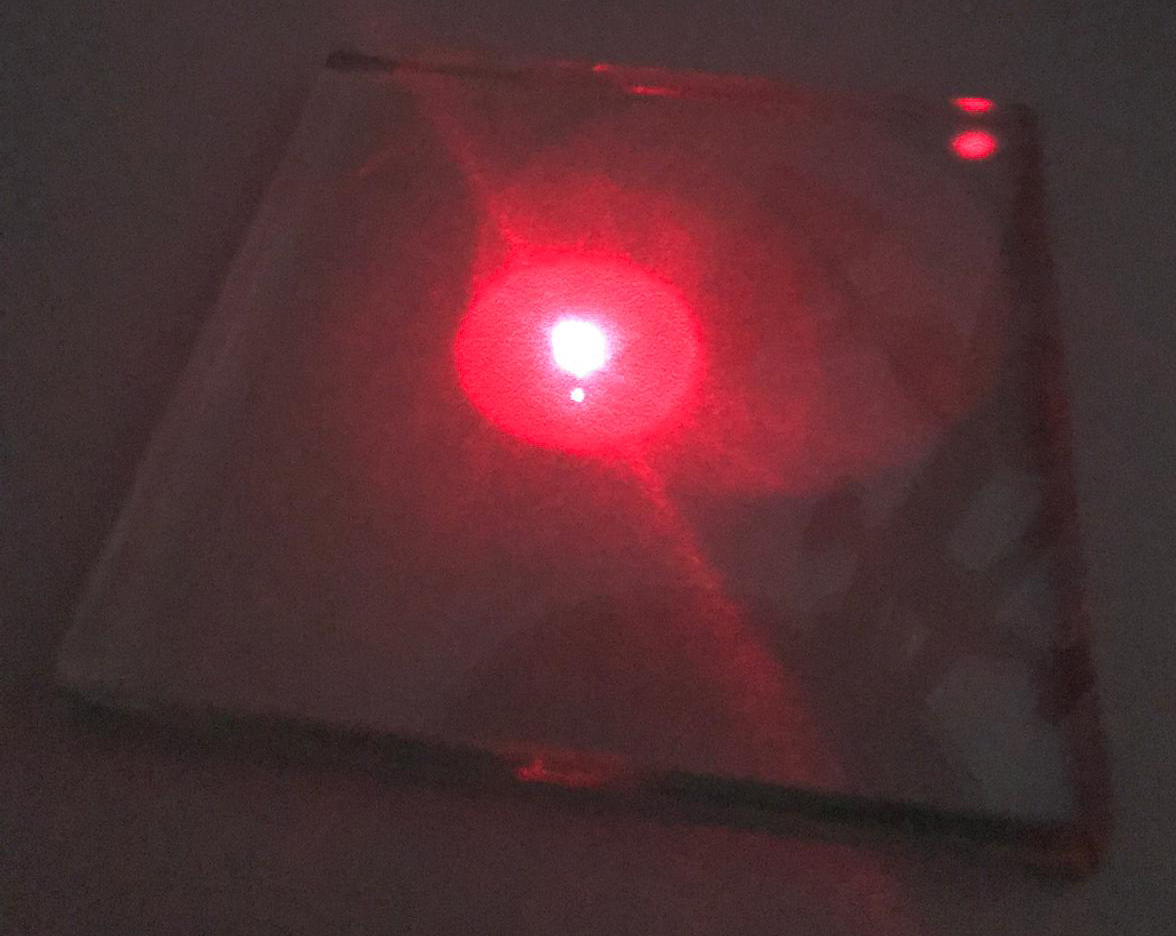
\includegraphics[width=7cm]{P2PffVidrio.jpeg}}
\subfigure{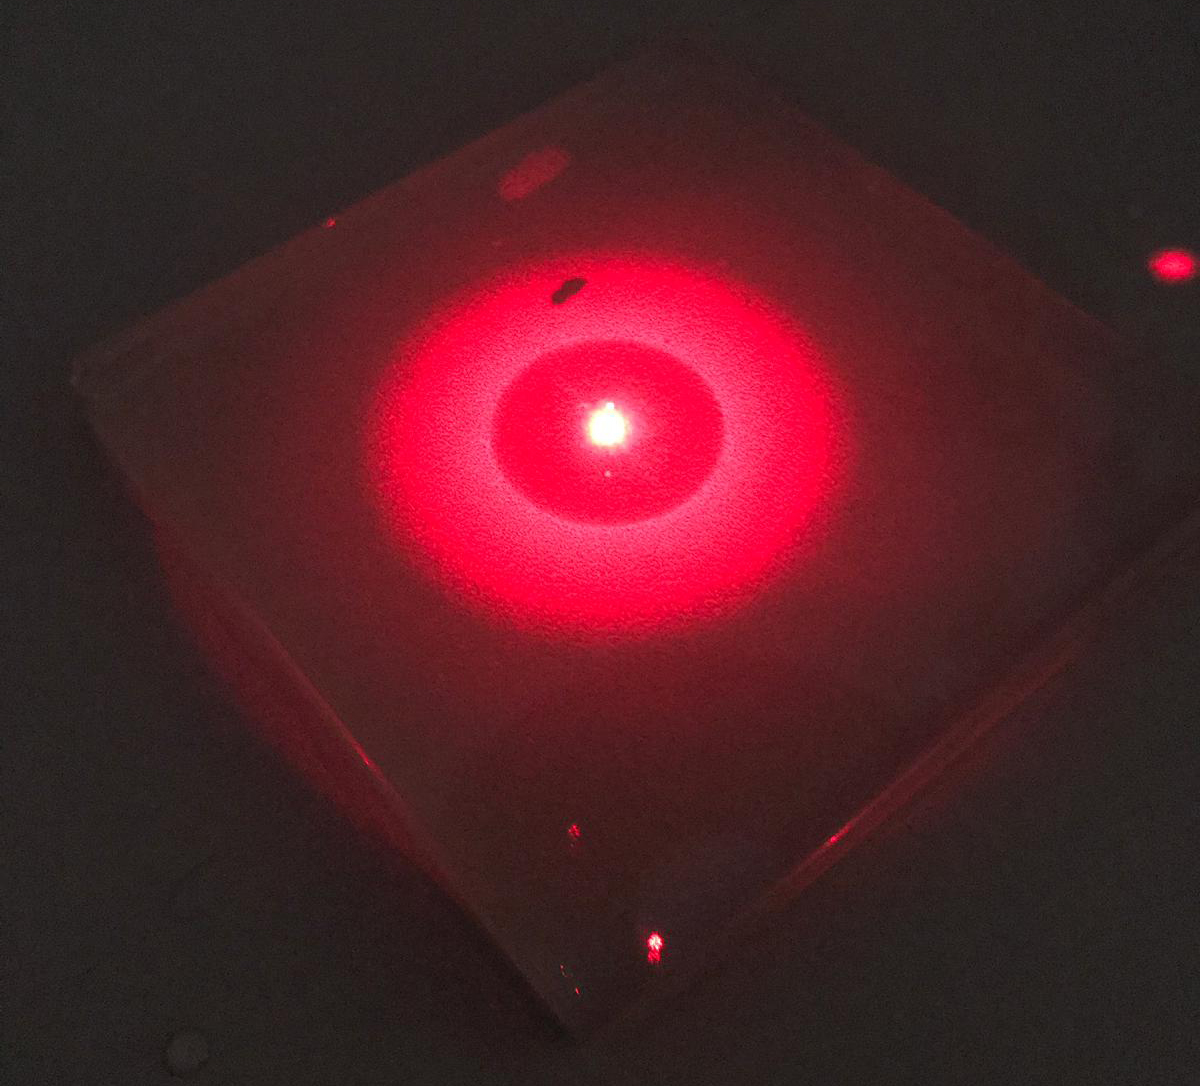
\includegraphics[width=6.15cm]{P2PffAgrio.jpeg}}
\caption{Dos fotografías de una lámina de vidrio sobre la mesa iluminada con un rayo láser ilustrando el efecto Pffund. En la derecha hay además una capa de agua entre el vidrio y la mesa.}
\label{P2PffFotoVidrio}
\end{center}
\end{figure}

Si debajo de la lámina de vidrio se pone una fina capa de agua, a los rayos que salen con menor inclinación que el ángulo límite les sucede lo mismo: mayoritariamente se refractan y en una pequeña parte se reflejan; pero los que salen con más que el ángulo límite al llegar a la superficie vidrio-aire se reflejan totalmente y cuando llegan a la superficie vidrio-agua, como el índice de refracción del agua es mayor que el del aire, el rayo se refracta casi totalmente y acaba llegando a la mesa, sobre la cual se refleja de forma difusa.

El índice de refracción del vidrio es mayor que el del agua. Por lo tanto si el rayo de luz llega suficientemente oblicuo ---con un ángulo $\varepsilon_l'$--- del vidrio al agua se puede producir reflexión total. Estos rayos vuelven a la superficie vidrio-aire y se vuelven a reflejar totalmente, quedándose atrapados y originando una zona oscura.

\begin{figure}[!ht]
\begin{center}
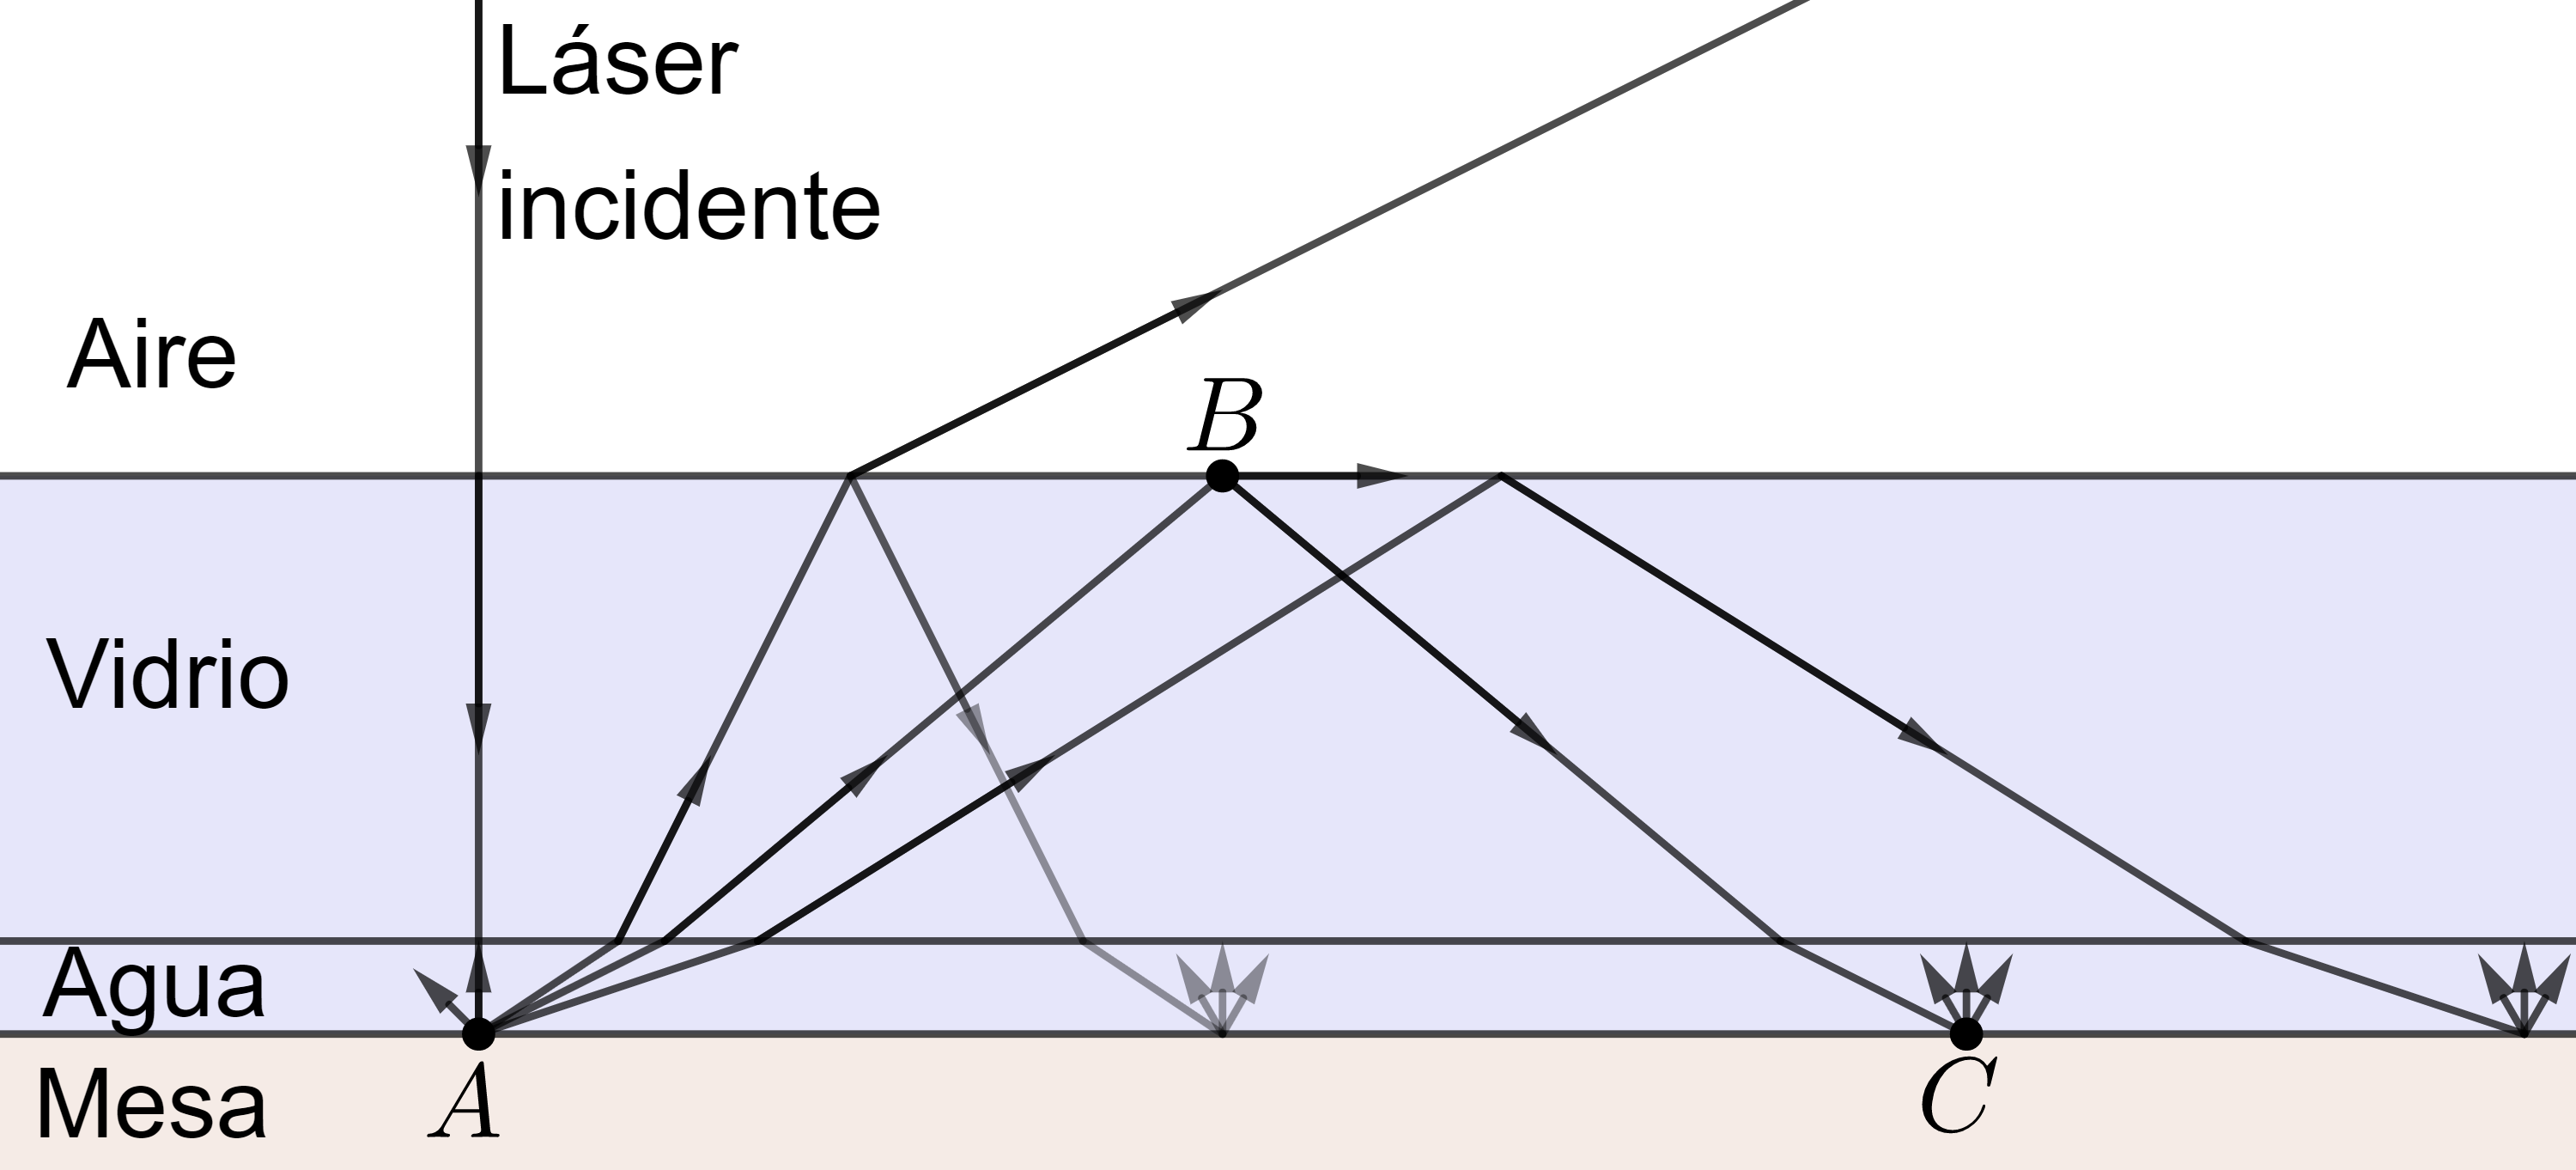
\includegraphics[width=10cm]{P2PffAgrio.png}
\caption{Esquema del efecto Pffund sobre una lámina de vidrio que reposa sobre una capa de agua.}
\label{P2PffAgrio}
\end{center}
\end{figure}

Se ve un punto central muy iluminado, una corona oscura a su alrededor, fuera de ella se ve una corona más grande iluminada y más allá de ella se queda oscuro. El radio de la corona oscura $r_1$ se calcula con la fórmula (\ref{P2PffRadioParvo}) siendo $n$ y $d$ los parámetros de la lámina de vidrio.

La corona iluminada se acaba donde el rayo de luz tiene un ángulo incidente $\varepsilon_l'$. $\sen\varepsilon_l'=\frac{n_\text{a}}{n_\text{v}}$. Con esto se puede calcular el radio de la corona oscura.

\begin{equation}\label{P2PffRadioMagno}
r=\frac{2d}{\sqrt{\left(\frac{n_\text{v}}{n_\text{a}}\right)^2-1}};\hspace{2mm}n_\text{a}=\frac{n_\text{v}}{\sqrt{1+\frac{16d^2}{\phi^2}}}
\end{equation}

Si hay una burbuja, los rayos que llegan a ella son desviados y la zona de donde salen estos se queda oscura. En lugar de ver el punto de donde salen los rayos, vemos la imagen de donde parecen venir los rayos, la cual vemos en otro lugar. Se puede ver esto en el esquema de la figura \ref{P2PffBurbuja}. El punto $A$ se ve perfectamente, pero el punto $O$ se ve oscuro porque en su lugar su imagen $O'$, que se debería ver oscura se ve iluminada.

\begin{figure}[!ht]
\begin{center}
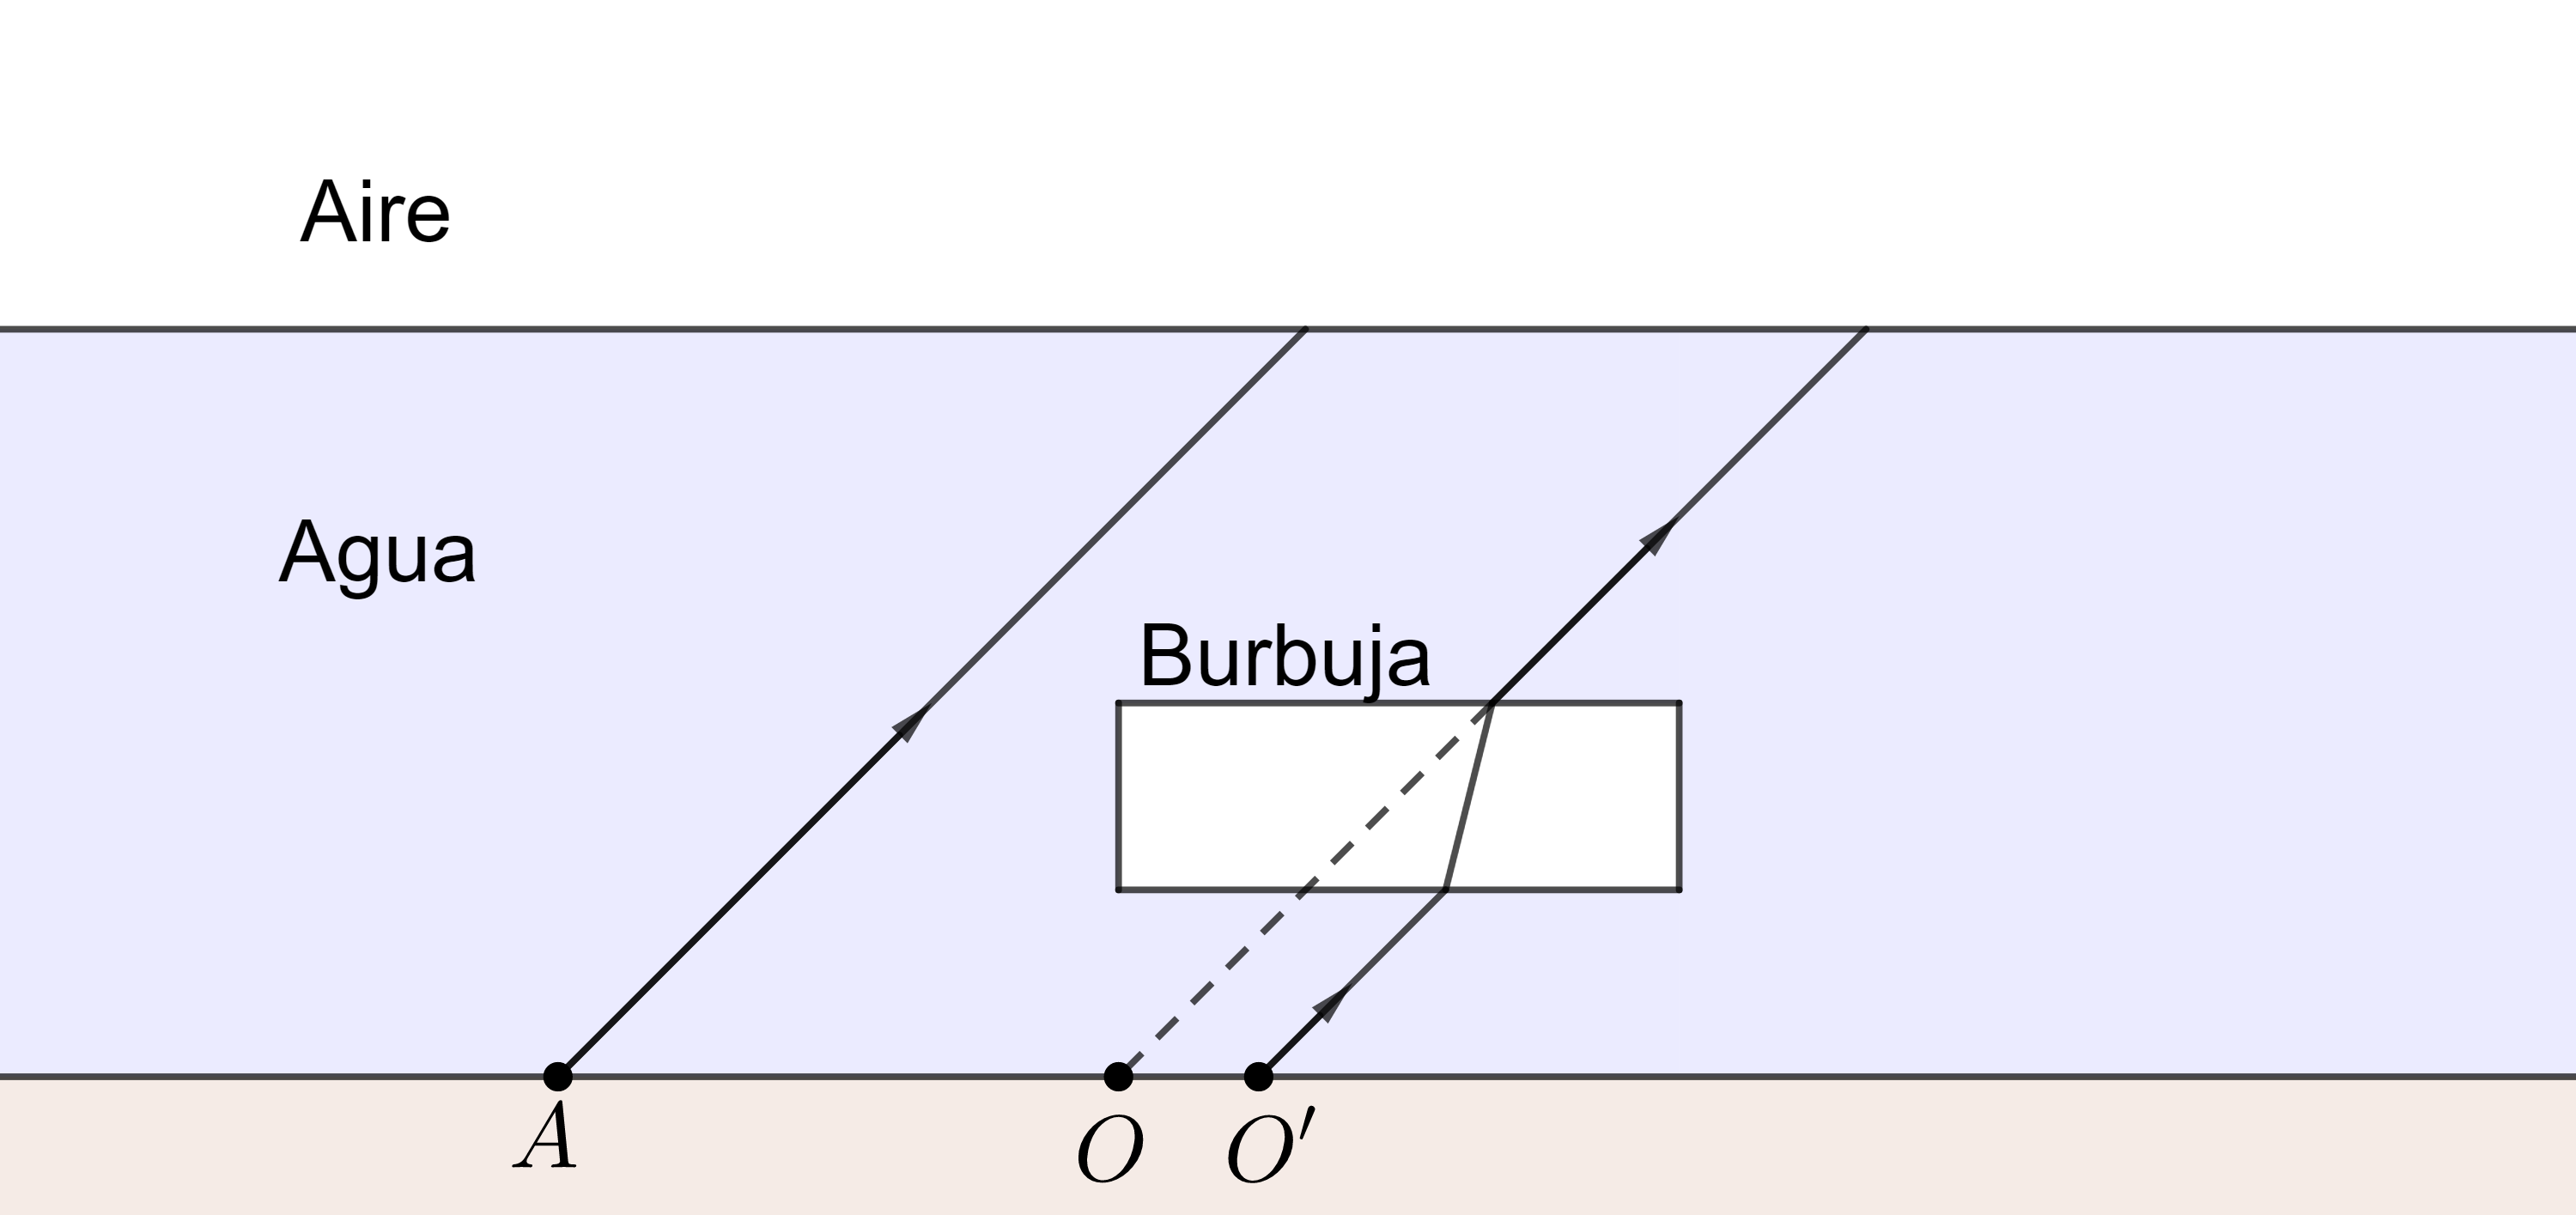
\includegraphics[width=10cm]{P2PffBurbuja.png}
\caption{Esquema del efecto de una burbuja sobre los rayos que llegan al ojo.}
\label{P2PffBurbuja}
\end{center}
\end{figure}

Una fotografía tomada de este caso y que confirma lo que se ha explicado se encuentra en la figura \ref{P2PffFotoVidrio}. Se ve el punto central brillante, una corona oscura y otra iluminada. Además se ve que hay una pequeña burbuja, pues los rayos que vienen de la mancha negra son desviados y parecen venir de la mancha iluminada que hay un poco más arriba en la imagen.
\\

Cuando se vierte agua sobre la lámina de vidrio el proceso que ocurre es el mismo, solo que el medio limítrofe con el aire es el agua, por lo que en la fórmula (\ref{P2PffRadioParvo}) del radio de la corona oscura se debe poner el índice de refracción del agua en lugar del del vidrio. Como los índices del agua y del vidrio son parecidos no se aprecia una gran diferencia en el radio. El radio de la corona iluminada, por su parte, permanece igual.

\begin{figure}[!ht]
\begin{center}
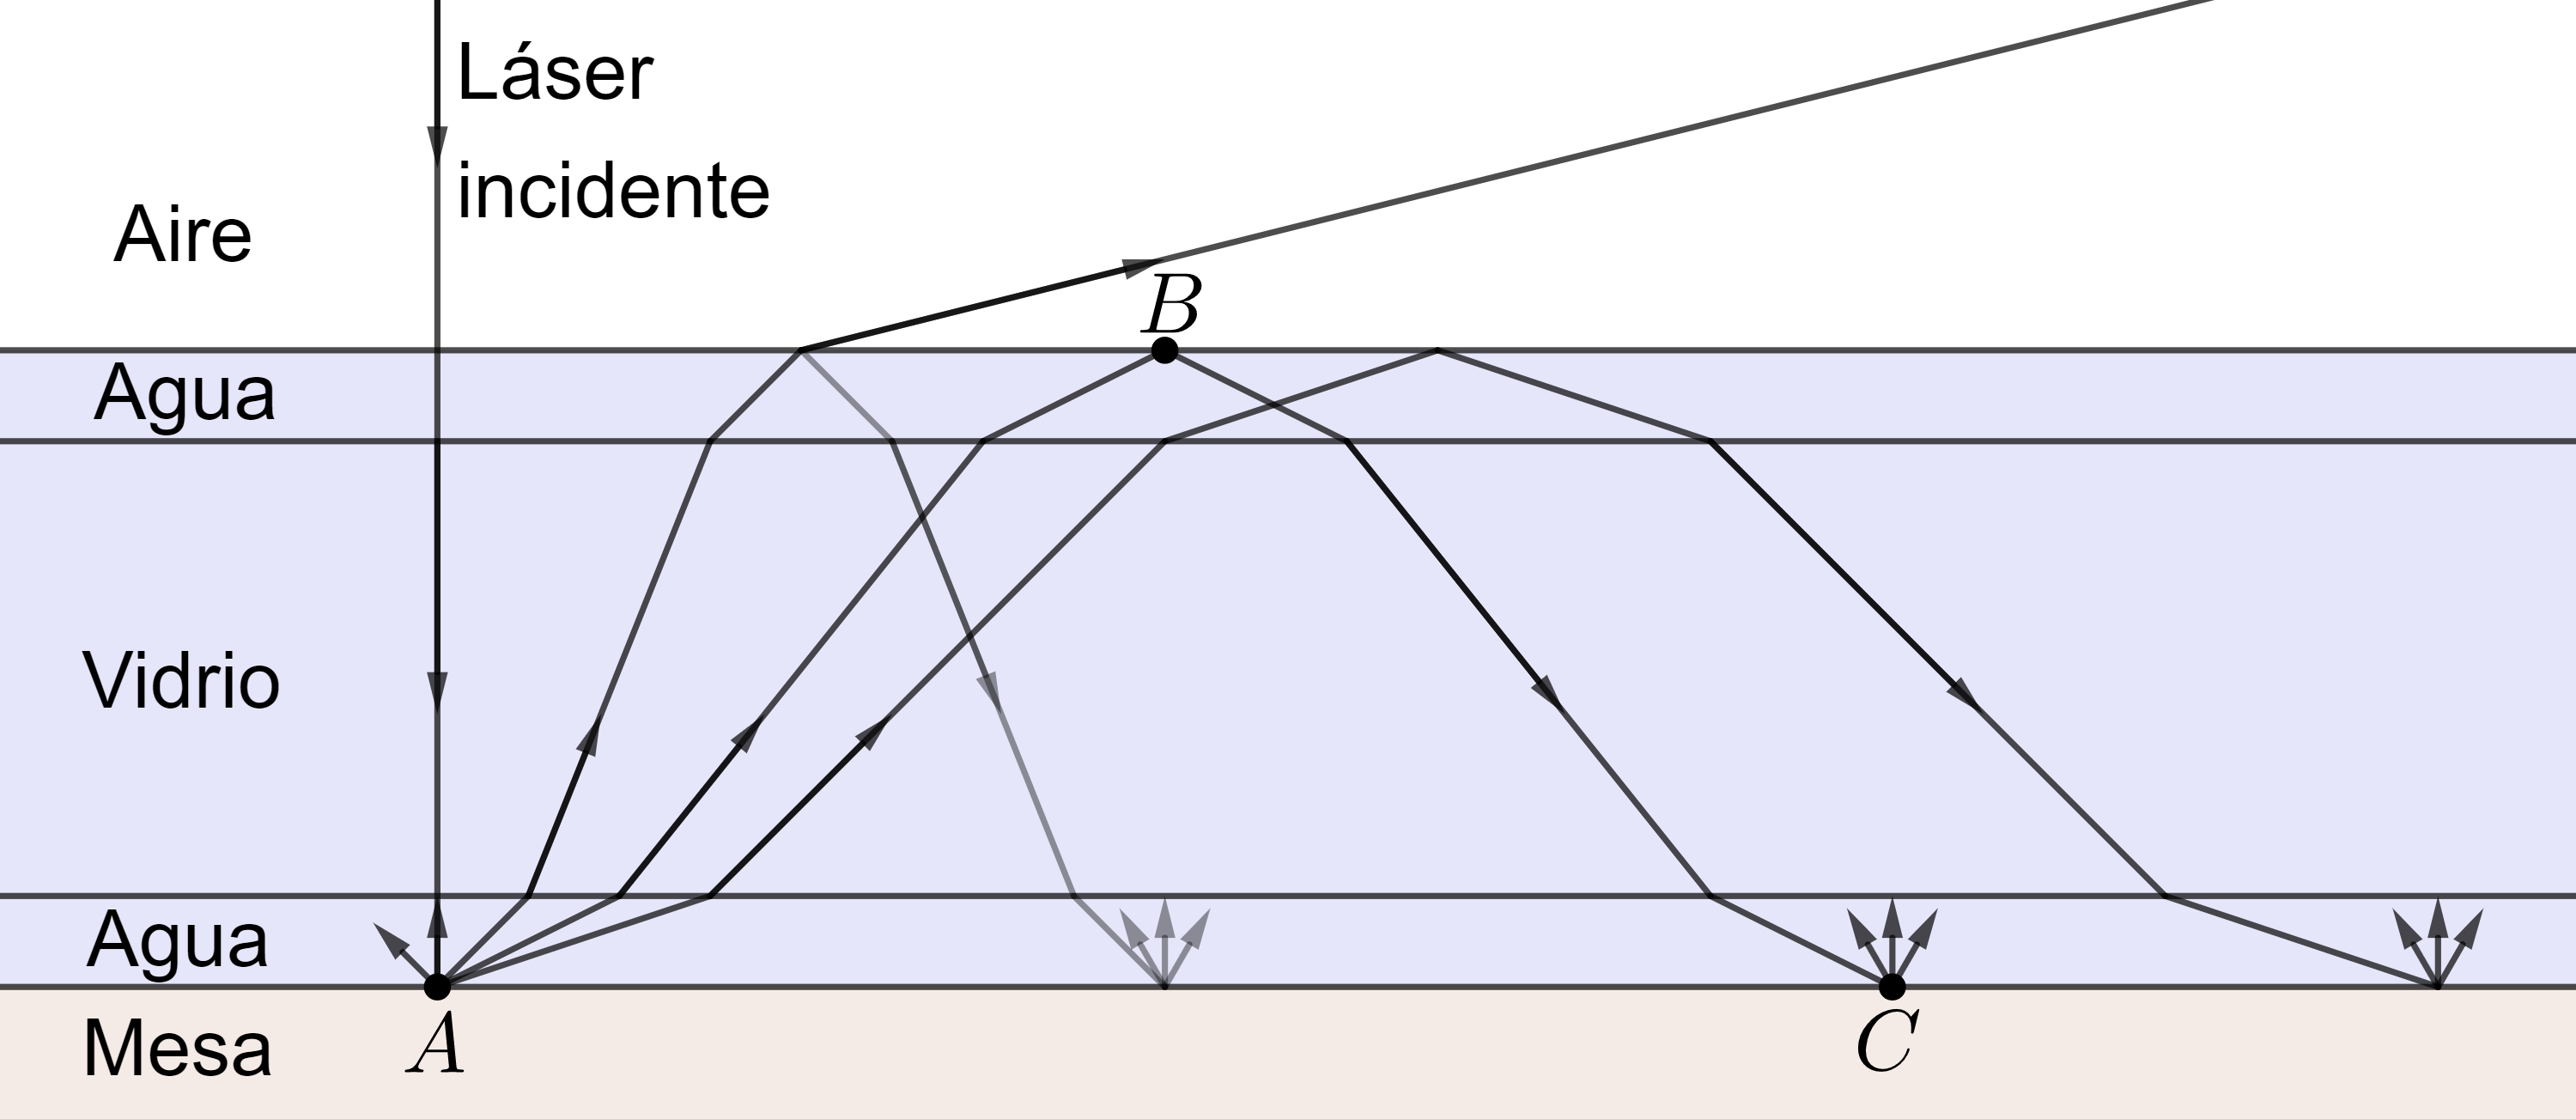
\includegraphics[width=10cm]{P2PffAgria.png}
\caption{Esquema del efecto Pffund sobre una lámina de vidrio que se encuentra entre dos capas de agua.}
\label{P2PffAgria}
\end{center}
\end{figure}

En cada caso han tenido lugar los siguientes fenómenos ópticos.
\begin{enumerate}
\item Luz sobre la mesa. Reflexión difusa.
\item Espejo por el lado de aluminio. Reflexión especular.
\item Papel satinado. Reflexión difusa y refracción.
\item Plástico. Reflexión difusa.
\item Espejo por el lado de vidrio. Refracción y reflexión especular.
\item Efecto Pffund.
\begin{itemize}
\item Reflexión difusa sobre la mesa
\item Reflexión especular en las superficies agua-aire, vidrio-aire, vidrio-agua.
\item Reflexión total del agua al aire, del vidrio al aire y del vidrio al agua.
\item Refracción en las superficies agua-aire, vidrio-aire, vidrio-agua.
\end{itemize}
\end{enumerate}

\subsection{Conclusiones}
En los fenómenos de refracción y reflexión de la luz, esta se puede entender como una serie de rayos que se propagan en línea recta, pues explican todos los resultados observados en esta práctica.

Cuando un objeto emite rayos que se refractan en un dioptrio plano, se forma una imagen que en el caso paraxial será nítida. Esta imagen es la que se ve con el ojo. Gracias a esto se ha podido calcular el índice de refracción de una lámina de vidrio. Se ha comprobado asimismo la dependencia del mismo con la longitud de onda de la luz empleada, lo cual genera una dispersión cromática, la cual en algunos casos no es despreciable y puede llegar a generar aberraciones cromáticas que impidan formar una imagen con claridad.
\\

Se ha visto también que no se ve el rayo de luz, sino el punto de donde proviene. Esto quiere decir que si un rayo sale de una fuente en una dirección y se refleja especularmente, pero no termina en el ojo, no se verá nada.

Además no todas las superficies son iguales: en algunas los rayos de luz se refractan, en otras se reflejan especular o difusamente, a veces una parte es refractada y otra reflejada... Esto da lugar al efecto Pffund, el cual utiliza conceptos de reflexión total y materiales de distintos índices de refracción para explicar las formas que se ven al iluminarlos. El efecto se ha podido comprobar satisfatoriamente en el laboratorio, permitiendo calcular los índices de refracción del vidrio y del agua.

Se puede concluir que la óptica geométrica es fundamental a la hora de explicar la propagación de la luz. Es capaz de explicar una gran cantidad de fenómenos que se producen cuando la luz llega a superficies de separación entre dos medios.

\section{Práctica 5. Polarización de la luz}
\subsection{Objetivos}
En esta práctica se pretende estudiar el fenómeno de la polarización de la luz, ---que muestra que la luz es una onda transversal---, y diversos modos de causarlo.

Se estudiará la polarización por absorción selectiva de diversos materiales, por reflexión, por dispersión Rayleigh en la luz proveniente del cielo y por birrefringencia en láminas retardadoras.

Por último se comprobará la ley de Malus para la intensidad de luz que atraviesa dos polaroides.

\subsection{Polarización por dicroísmo}
La polarización por dicroísmo tiene lugar cuando la luz atraviesa una lámina de un material que absorbe una componente y transmite la perpendicular. Normalmente estas láminas consisten en cadenas rectilíneas de moléculas que permiten a los electrones moverse en una sola dirección. Si esta dirección es la vertical, los electrones interactuarán con la componente de la onda cuyo campo eléctrico oscile en el eje vertical, pues el que oscila en el eje horizontal no puede ejercer trabajo sobre los electrones, ya que estos no se desplazan en la dirección horizontal. Así pues los electrones de la lámina absorben la componente vertical del campo eléctrico y transmiten la componente horizontal.

Se apunta a una pantalla con una fuente de luz y se coloca un polarizador HN-22 entre ambas. El resultado es una leve disminución de la intensidad de la luz que llega a la pantalla. Al girar el polarizador no se observa ningún cambio, pues se está cambiando la dirección de polarización de la luz que llega a la pantalla pero no su intensidad.

La disminución de intensidad es un indicio de que la luz se ha polarizado, pero no es una prueba, pues podría por ejemplo absorberse una fracción de la luz igual para todas las direcciones. Para comprobar que efectivamente la luz sale polarizada se coloca entre el polaroide y la pantalla otro polaroide HN-38. al girar el segundo polaroide la intensidad va aumentando y disminuyendo. Cuando la pantalla está oscura es porque los ejes de transmisión de ambos polaroides son perpendiculares. El primer polaroide deja pasar luz únicamente en una dirección, que es justo la dirección que absorbe el segundo. Por lo tanto no llega luz a la pantalla y se ve oscura. Sin embargo, la oscuridad no es total, ya que los polarizadores no son ideales: tansmiten un poco de luz en la dirección de absorción y viceversa. Este fenómeno pone en evidencia que la luz que sale de los polaroides está efectivamente polarizada.

Ahora se cambia el polaroide HN-38 por uno HN-22, de manera que los dos polariodes tienen las mismas curvas de transmitancias. Estas curvas se encuentran en la figura \ref{P5transmitancias}. En este caso cuando los ejes de transmisión son perpendiculares se ve una oscuridad más intensa porque la transmitancia del polaroide HN-22 en el eje de absorción es mucho menor que la del HN-38. La intensidad cuando los ejes son paralelos es parecida con el polaroide HN-38 y el HN-22 porque tienen transmitancias similares en el eje de transmisión.

\begin{figure}[!ht]
\begin{center}
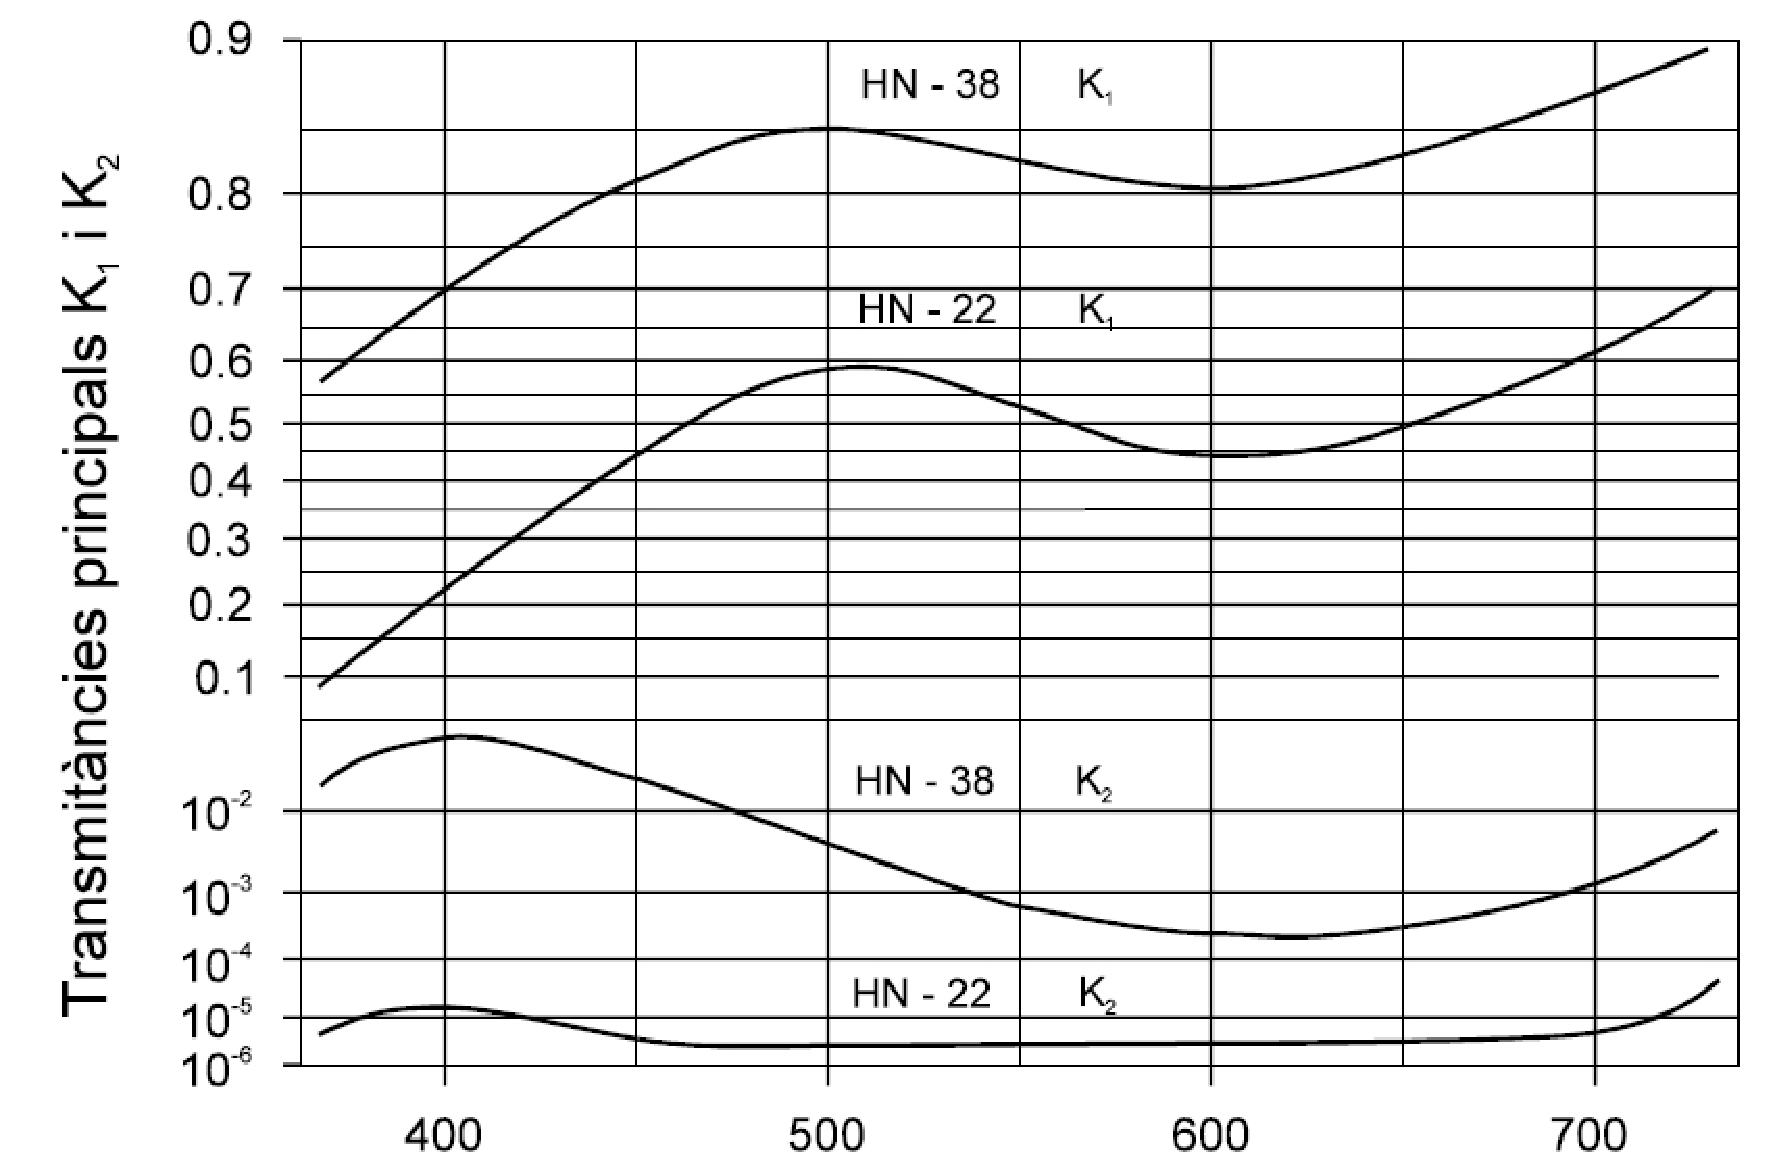
\includegraphics[width=10cm]{P5Transmitancias.pdf}
\caption{Gráficas de las transmitancias principales $K_1$ y $K_2$ en los ejes de transmisión y absorción respectivamente de los polarizadores HN-22 y HN-38 en función de la longitud de onda.}\label{P5transmitancias}
\end{center}
\end{figure}

Uno de los polarizadores tiene el eje de transmisión marcado. El eje de transmisión del otro se puede determinar girándolo hasta obtener la posición en la que la intensidad que llega a la pantalla es mínima. En este punto el eje de transmisión es el perpendicular al del otro polarizador ---cuyo eje de transmisión es conocido---. Este método es más preciso que girar el polarizador hasta obtener intensidad máxima ---siendo igual la dirección de transmisión de ambos polaroides--- porque se determina con mayor exactitud el ángulo de intensidad mínima que la máxima.

En la figura \ref{P5transmitancias} se ve que las transmitancias dependen de la longitud de onda. Para poner de manifiesto esta dependencia se colocan un filtro verde y otro rojo en la fuente de luz. Cuando los ejes son paralelos no se ve mucha diferencia, pero cuando son perpendiculares la luz que llega a la pantalla es menos intensa con el filtro verde que con el rojo. Si observamos la curva de $K_1$ del HN-22 la transmitancia es similar para longiudes de onda alrededor de los $\unit[500]{nm}$ (verde) y de los $\unit[700]{nm}$ (rojo). Sin embargo $K_2$ es bastante mayor para el rojo que el verde (obsérvese que del $10^{-1}$ hacia abajo la escala es logarítmica: pequeños cambios en el eje $y$ son grandes cambios de transmitancia).

Ahora se disponen los polarizadores con los ejes de transmisión cruzados y se colocan objetos entre ambos polarizadores. Se coloca asimismo una lente para proyectar los objetos sobre la pantalla. Este sistema se llama polariscopio.

Si se pone una lámina de vidrio no ocurre nada. La luz sale del vidrio tal cual ha entrado. No cambia su polarización. Por lo tanto se ve oscura la pantalla. Si se pone papel, sin embargo, sí que se ve algo de luz porque la luz polarizada que llega al papel se dispersa en él y sale despolarizada. Así la luz que llega al segundo polarizador tiene una componente no nula en el eje de transmisión. Independientemente de la orientación del papel o de los polarizadores se ve lpantalla iluminada.

Cuando se pone celofán se ilumina la pantalla según el ángulo de orientación. Cuando se gira se puede conseguir que se ilumine la pantalla. Si se orienta para ver el máximo de intensidad, para que vuelva a dejar de pasar la luz se ha de girar 90º. Esto se explica porque el celofán cambia la orientación de la polarización de la luz, de modo que si antes llegaba la luz oscilando perpendicular al eje de transmisión del segundo polarizador, con el celofán se puede cambiar la orientación de la polarización para que la luz llegue al segundo polarizador con el campo eléctrico oscilando en la dirección de transmisión.

También se puso una pequeña lámina de plástico con varios trozos de cinta adhesiva simple. Se observaron los distintos trozos de diferentes colores como muestra la figura \ref{P5colorines}. El celo modifica la orientación de la polarización de la luz, pero no afecta todas las longitudes de onda por igual: cada una gira su polarización por separado. Por eso algunas longitudes de onda llegan paralelas al eje de transmisión proyectándose sobre la pantalla y otras llegan perpendiculares siendo absorbidas. Además cada capa modifica la polarización y por lo tanto según la cantidad de capas de cinta que haya se ve de un color u otro. Al girar el plástico se ve cómo cambian los colores.

\begin{figure}[!ht]
\begin{center}
\subfigure{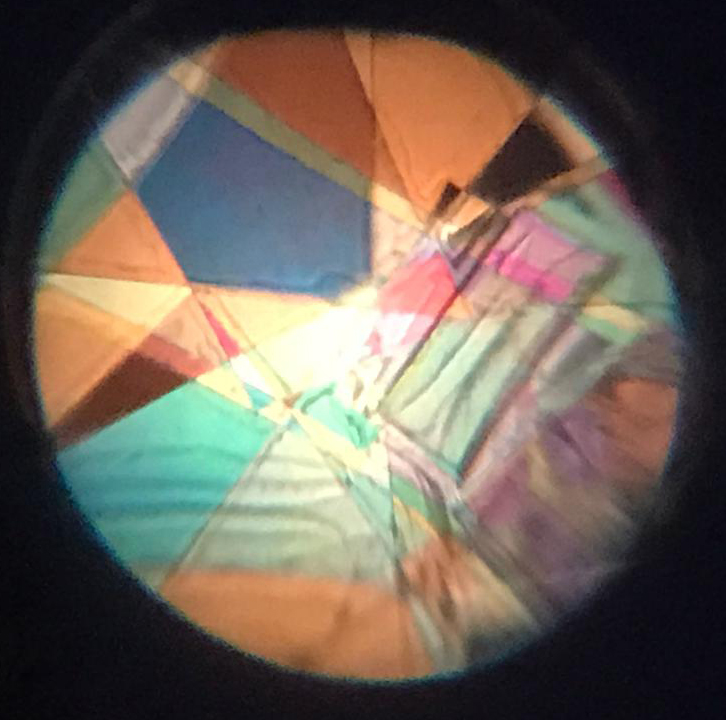
\includegraphics[width=6.72cm]{P5Celo1.jpg}}
\subfigure{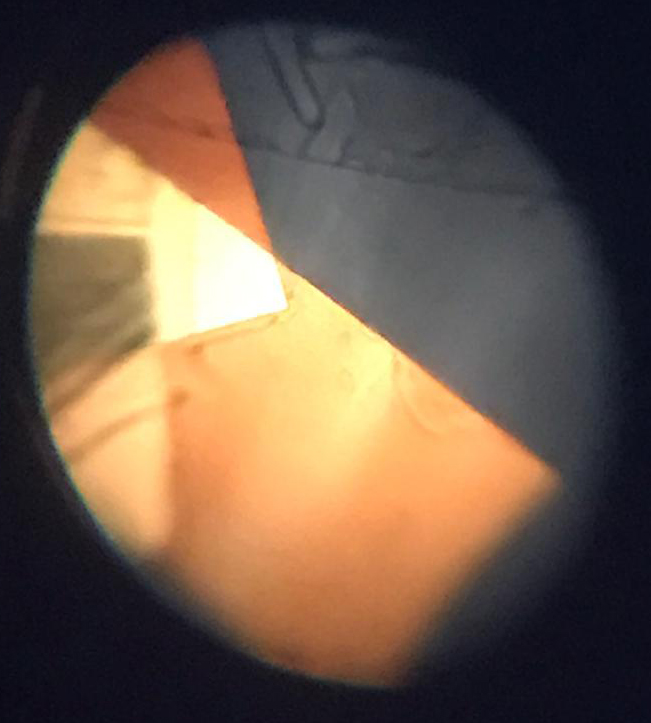
\includegraphics[width=6cm]{P5Celo2.jpg}}
\caption{Fotografías de la la pantalla con cinta adhesiva en el polariscopio.}\label{P5colorines}
\end{center}
\end{figure}

Por último se coloca una caja de un CD, que es un plástico rígido, en el polariscopio. Se observan diversos colores en la pantalla como con la cinta adhesiva. Al presionar el plástico, los colores cambian, lo cual se puede explicar porque al sufrir esfuerzos el plástico cambia la orientación de las diversas longitudes de onda de la luz polarizada.

\section{Práctica 10. Efecto fotoeléctrico}
\subsection{Objetivos}
En esta práctica se pretende estudiar el efecto fotoeléctrico, que consiste en la liberación de electrones ligados a un metal por la acción de una luz incidente. Se evaluará cómo influyen en este proceso la intensidad de la luz, su longitud de onda, etc.

Esta práctica ayudará a entender el comportamiento corpuscular de la luz y los motivos que llevaron a Einstein a proponerlo. Se pretende averiguar si las predicciones del modelo corpuscular de Einstein se ajustan a los datos que se obtengan.

Posteriormente este fenómeno físico será utilizado para estimar la constante de Planck, que es la constante fundamental de toda la física cuántica.

\subsection{Cuestiones teóricas}
El efecto fotoeléctrico se produce cuando se ilumina una placa metálica llamada cátodo y se arrancan electrones que van otra placa llamada ánodo. En el modelo que propuso Einstein la luz está formada por corpúsculos a los que llamó fotones. Cada uno de estos fotones tiene una energía que depende de su frecuencia de oscilación.
\begin{equation}\label{P10Efoton}
E_{\text{fotón}}=h\nu
\end{equation}
$h$ es la constante de Planck y $\nu$ es la frecuencia.

Cuando un fotón incide sobre el metal, es absorbido enteramente por un electrón que está orbitando en un átomo. Cada electrón absorbe un único fotón de vez. Así cuando un fotón es absorbido por un electrón, toda su energía es transferida al electrón, el cual invierte una parte en trabajo para desligarse del átomo, $q_e\Phi$, y otra se queda en forma de energía cinética $E_c$.
\begin{equation}\label{P10ecuacion}
h\nu=q_e\Phi+E_c
\end{equation}
Si se quiere extraer un electrón, la mínima energía necesaria para hacerlo es cuando la energía cinética es 0. $h\nu=q_e\Phi$.

Si se quisiese extraer un electrón de un fotocátodo de sodio, cuya función de trabajo es $\unit[2.27]{eV}$, la frecuencia mínima que habría que aplicarle sería $\nu_{\text{mín}}=\frac{q_e\Phi}{h}=\frac{\unit[2.27]{eV}}{\unit[4.14\cdot10^{-15}]{eV\cdot s}}=\unit[5.49\cdot10^{14}]{Hz}$, que es aproximadamente la frecuencia del verde.
\\

Al aumentar la frecuencia del fotón, por la ecuación (\ref{P10Efoton}), aumenta su energía y por la ecuación (\ref{P10ecuacion}), ---en el caso en que la energía del fotón es suficiente para arrancar el electrón---, aumenta la energía cinética del electrón, pues la función de trabajo permanece constante. Esto ocurre porque un fotón es absorbido enteramente por un electrón, es decir, la energía del fotón se transmite íntegra a un único electrón, no se divide en varios.

Al aumentar la intensidad manteniendo la frecuencia constante se está incrementando la cantidad de fotones que inciden sobre la placa metálica, pero no la energía de cada uno de estos. Cada electrón absorbe un único fotón, de modo que la energía que tenga el electrón después de absorberlo será independiente de la cantidad de fotones incidentes. Así pues, no variará su energía cinética; lo que variará será la cantidad de electrones extraídos.
\\

Si se pone un voltaje de frenado entre el fotocátodo y el fotoánodo, disminuirá la energía de los electrones. $h\nu=E_c+q_eV+q_e\Phi$. En esta práctica se buscará el voltaje que frene los electrones totalmente, de modo que su energía cinética en en el fotoánodo sea nula.
\begin{equation}\label{P10regresion}
V=\frac{h}{q_e}\nu-\Phi
\end{equation}
La lámpara con que se ilumina la fotocélula es de corriente alterna, de modo que la intensidad que genera varía periódicamente con el tiempo. Por lo tanto la componente de la señal eléctrica generada por la fotocélula será alterna. No obstante, también se generará una componente continua debida al ruido ambiente (radiación residual que hay en el laboratorio).

El circuito en el que se encuentra la fotocélula hay un amplificador que amplifica únicamente la componente alterna con el fin de minimizar el ruido y observar con mejor precisión la señal de la luz proveniente de la lámpara, que es de la que se pueden controlar parámetros como la frecuencia o la intensidad.

\subsection{Análisis cualitativo}
%Explicar mejor
Al principio se enciende el osciloscopio y se observa la señal que aparece en su pantalla. Esta es una señal muy débil que corresponde al ruido electromagnético presente en el aire. Cuando se aprietan con los dedos los extremos de los cables a los que se conecta el osciloscopio, se observa un leve incremento de la señal.
\\

Ahora se conecta la lámpara con un filtro de color ---sin importar cuál sea---. La lámpara está conectada a un enchufe, que transmite una corriente alterna de $\unit[50]{Hz}$, de modo que el voltaje y la intensidad variarán con esa frecuencia. El voltaje $V=V_0\sen\omega t$ y la intensidad $I=I_0\sen\omega t$ están en fase. Esta última se representa en la figura \ref{P10intensidadfilamento}. El filamento de tungsteno se calienta por efecto Joule con una potencia $P=IV=P_0\sen^2\omega t$. Su frecuencia es el doble que la de la intensidad porque el filamento se calienta de igual modo cuando la corriente va en un sentido que cuando va en el otro. Se calienta cuando la intensidad tiene un pico (tanto máximo como mínimo) y se enfría cuando la intensidad es 0. La temperatura varía aproximadamente junto con la potencia y se puede ver en la figura \ref{P10temperatura}.

Por la ley de Stefan-Boltzmann, la potencia que emite un cuerpo ---no necesariamente negro--- es igual al producto de su emisividad, la constante de Stefan-Boltzmann y la cuarta potencia de la temperatura. La intensidad luminosa que llega a la fotocélula es proporcional a la potencia de radiación emitida por la lámpara y viene representada en la figura \ref{P10intensidadluminosa}. Se puede observar que los picos de intensidad máxima son más acusados como consecuencia de elevar a la cuarta. La intensidad eléctrica generada en la fotocélula es proporcional a la cantidad de electrones arrancados del fotocátodo, que a su vez es proporcional a la intensidad luminosa en él incidente. Su dependencia temporal está representada en la figura \ref{P10intensidadfotocelula}.

Como consecuencia de todo esto, la intensidad de corriente eléctrica generada en la fotocélula tendrá forma parecida a una sinusoide con el doble de frecuencia que la corriente eléctrica doméstica, es decir, $\unit[100]{Hz}$.
\\

\begin{figure}[!ht]
\begin{center}
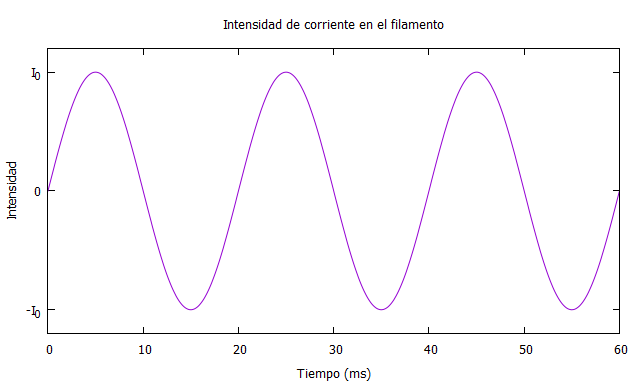
\includegraphics[width=10cm]{P10Intensidadfilamento.png}
\caption{Esquema de la intensidad de corriente eléctrica que circula por el filamento de la lámpara en función del tiempo.}\label{P10intensidadfilamento}
\end{center}
\end{figure}
\begin{figure}[!ht]
\begin{center}
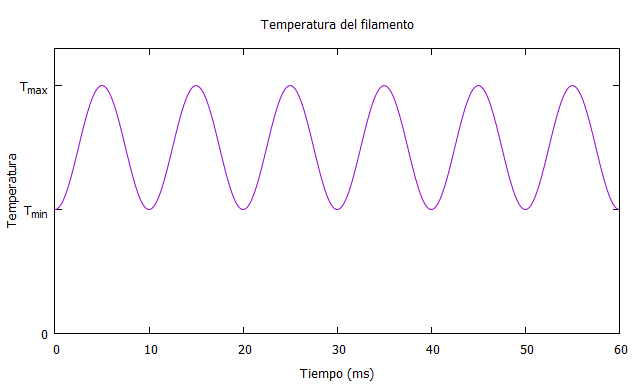
\includegraphics[width=10cm]{P10Temperatura.png}
\caption{Esquema de la temperatura del filamento de la lámpara en función del tiempo.}\label{P10temperatura}
\end{center}
\end{figure}
\begin{figure}[!ht]
\begin{center}
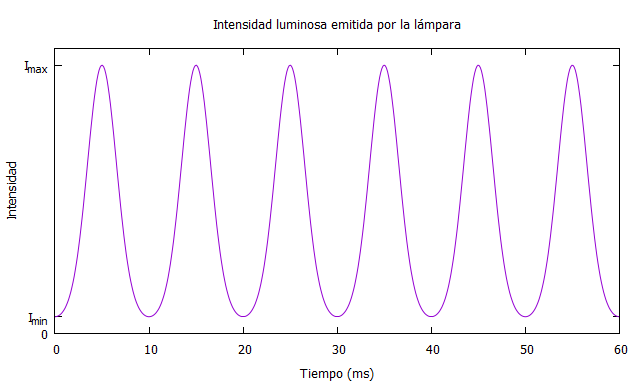
\includegraphics[width=10cm]{P10Intensidadluminosa.png}
\caption{Esquema de la intensidad luminosa que emite el filamento de la lámpara en función del tiempo.}\label{P10intensidadluminosa}
\end{center}
\end{figure}
\begin{figure}[!ht]
\begin{center}
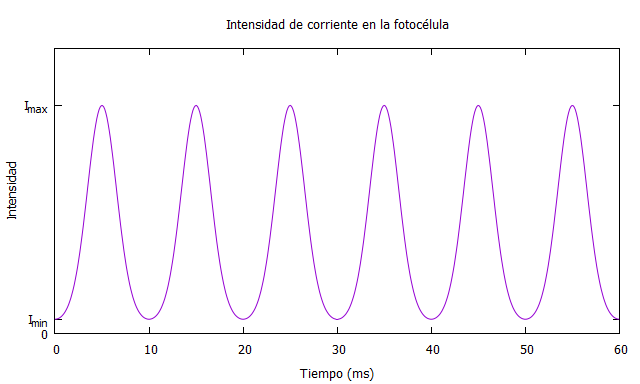
\includegraphics[width=10cm]{P10Intensidadfotocelula.png}
\caption{Esquema de la intensidad de corriente eléctrica que atraviesa la fotocélula en función del tiempo.}\label{P10intensidadfotocelula}
\end{center}
\end{figure}

Al medir la señal producida por la fotocélula y que llega al osciloscopio, se observa que es una onda periódica con período $\unit[(10\pm1)]{ms}$. Su frecuencia es la inversa del período y es $\unit[(100\pm10)]{Hz}$, tal como se había predicho.

\subsection{Análisis cuantitativo}
En esta parte de la práctica se mide el voltaje de frenado  necesario para detener los electrones antes de que lleguen al fotoánodo. Para ello se mira con el osciloscopio la señal de la célula fotoeléctrica y se va aumentando el potencial de frenado hasta que la señal del osciloscopio se hace plana. En ese momento el potencial que se está aplicando entre las dos placas es el que aparece en la ecuación (\ref{P10regresion}). Se repite el proceso para varios filtros de diversas frecuencias. Cuanto mayor sea la frecuencia, tanto mayor será la energía de los electrones arrancados y por ende mayor se espera que sea el voltaje de frenado.

Cada filtro tiene toda una curva de transmisión para el espectro electromagnético. Esta curva tiene un pico alrededor de una cierta longitud de onda, pero también transmite otras longitudes, aunque con menos intensidad. Sin embargo a la hora de asignar una longitud de onda a un filtro también se ha de tener en cuenta que el espectro de emisión de la lámpara no es uniforme: es mayor en el centro de la parte visible y menor cerca del ultravioleta y del infrarrojo. En cada filtro se elige una longitud de onda que esté cerca del máximo de transmisión y que la lámpara emita con una intensidad suficiente.

En las gráficas de transmisión en función de la longitud de onda de los filtros, el eje x está dividido en intervalos de $\unit[5]{nm}$, que se coge como incertidumbre de $\lambda$. La frecuencia se calcula con la expresión $\lambda\nu=c$ y su incertidumbre con la fórmula de propagación de errores.
\\

Al medir el voltaje de frenado, el voltaje que marca la ruleta del aparato que aplica el potencial regulable coincide con el medido con un polímetro, pero en este último se tiene más precisión, de modo que se coge el valor que marca el polímetro.
\begin{figure}[!ht]
\begin{center}
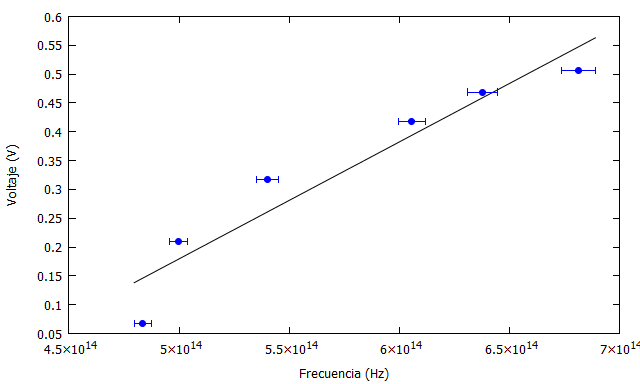
\includegraphics[width=10cm]{P1016,3cm.png}
\caption{Representación del voltaje entre las placas en función de la frecuencia de la radiación con la lámpara a una altura de $\unit[16.3]{cm}$. Se incluye la recta de regresión lineal de pendiente $\unit[(2.03\pm0.32)\cdot10^{-15}]{V/Hz}$ y de ordenada en el origen $\unit[(-0.83\pm0.18)]{V}$. El coeficiente de correlación es $0.910$.}
\label{P1016,3cm}
\end{center}
\end{figure}
\begin{figure}[!ht]
\begin{center}
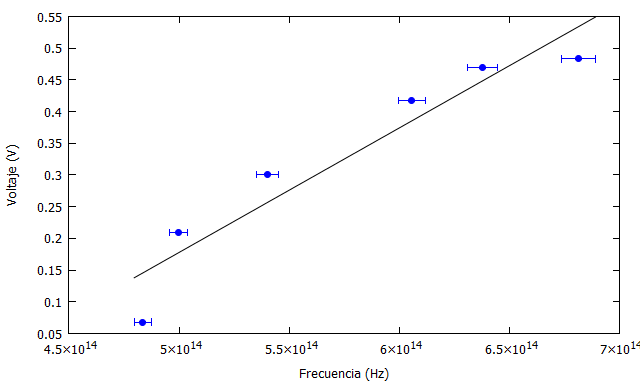
\includegraphics[width=10cm]{P1023,5cm.png}
\caption{Representación del voltaje entre las placas en función de la frecuencia de la radiación con la lámpara a una altura de $\unit[23.5]{cm}$. Se incluye la recta de regresión lineal de pendiente $\unit[(1.96\pm0.32)\cdot10^{-15}]{V/Hz}$ y de ordenada en el origen $\unit[(-0.80\pm0.19)]{V}$. El coeficiente de correlación es $0.903$.}
\label{P1023,5cm}
\end{center}
\end{figure}
En las figuras \ref{P1016,3cm} y \ref{P1023,5cm} se ve el voltaje de frenado medido con filtros de distintas frecuencias, así como la recta de regresión a la que ajustan los puntos experimentales. En la primera gráfica la lámpara se encuentra a $\unit[16.3]{cm}$ y en la segunda a $\unit[23.5]{cm}$. Se observa claramente que los voltajes son muy similares en ambos casos y las rectas de regresión también. Esto es así porque cuando se mueve la lámpara de posición se está variando la intensidad con que la radiación llega a la fotocélula. Cuanto más alejada se encuentra la lámpara, menor es la intensidad con que llega la luz como consecuencia de la atenuación. Sin embargo las frecuencias de la luz al incidir sobre la fotocélula son las mismas, pues dependen de los filtros y se han usado los mismos en ambos casos.

Como se ha explicado anteriormente, si se varía la intensidad pero no la frecuencia de la radiación incidente, se cambia la cantidad de electrones que son arrancados, pero no su energía. El voltaje de frenado depende únicamente de la energía con que salen los electrones, no de la cantidad de estos. Por eso las gráficas son similares; varían únicamente en pequeñas componentes aleatorias al realizar las medidas. De hecho esta independencia de la intensidad se ve de forma matemática en la relación (\ref{P10regresion}), donde no aparece la intensidad.

El coeficiente de correlación lineal es cercano a 1, aunque quizá no demasiado. Además se ve que la recta de regresión lineal no entra dentro de las incertidumbres de los puntos. Esto se debe a que la incertidumbre que se ha cogido es demasiado pequeña. De hecho la incertidumbre del voltaje es más pequeña que el grosor de los puntos y no se ve. Hay todo un rango de voltajes en los que la señal del osciloscopio parece ser 0, de manera que la incertidumbre del voltaje es mayor que únicamente la precisión del polímetro. Además está el ruido que, aunque es disminuido por el amplificador, aún interfiere en la señal y hace que no se mida el valor exacto del voltaje. Por su parte la elección de la longitud de onda es un poco arbitraria: donde parece que coinciden una gran transmisión del filtro con una gran emisión de la lámpara. Sin embargo esta decisión es muy aproximada y a la hora de tomar la incertidumbre se está cogiendo únicamente la longitud de cada división del eje x en las gráficas.

Todo esto genera un cierto error y hace que el coeficiente de correlación no sea tan cercano a 1 como se podría esperar ---aunque sí que se acerca---.
\\

Con la recta de regresión se pueden calcular la función de trabajo del metal del fotocátodo y la constante de Planck. En la ecuación de la recta (\ref{P10regresion}) se ve que la ordenada en el origen es $n=-\Phi=-\frac{q_e\Phi}{q_e}$ donde $q_e\Phi$ es la función de trabajo. También se tiene la pendiente $m=\frac{h}{q_e}$. Se pueden despejar los valores de $h$ y $q_e\Phi$. Sus incertidumbres se calculan con la fórmula de propagación de incertidumbres. El  valor verdadero de la constante de Planck es $\unit[6.626\cdot10^{-34}]{J\cdot s}$ y el de la carga eléctrica del electrón es $\unit[1.602\cdot10^{-19}]{C}$.

Con la lámpara a $\unit[16.3]{cm}$ se tiene una función de trabajo $q_e\Phi=\unit[(1.34\pm0.30)\cdot10^{-19}]{J}$ una constante de Planck $h=\unit[(3.25\pm0.51)\cdot10^{-34}]{J\cdot s}$. Es aproximadamente la mitad del valor verdadero; su discrepancia es del $51\%$.

Con la lámpara a $\unit[23.5]{cm}$ la función de trabajo calculada experimentalmente vale $q_e\Phi=\unit[(1.29\pm0.30)\cdot10^{-19}]{J}$ y la constante de Planck experimental es $h=\unit[(3.15\pm0.52)\cdot10^{-34}]{J\cdot s}$ con un discrepancia del $53\%$. Los datos experimentales son bastante dispares con el valor de la constante. Esto es debido a lo comentado anteriormente, sumado a una posible mala calibración del aparato con que se estudia el efecto fotoeléctrico.
\\
\\

Cuando se aumenta la diferencia de potencial entre el fotocátodo y el fotoánodo más allá del voltaje de frenado en el cual los electrones se detienen totalmente, se vuelve a ver una señal sinusoidal como la que se veía sin poner un voltaje de frenado, similar a la de la figura \ref{P10sinusoide}.

Este fenómeno podría ser debido a que los electrones no solo salieran del fotocátodo y llegaran al fotoánodo, sino que también hubiera electrones que viajaran al revés: la luz que incide sobre el fotoánodo arrancase de ahí electrones que fueran a parar al fotocátodo. Para comprobar esta hipótesis se tapará el fotoánodo, de modo que solo haya electrones viajando del cátodo al ánodo. Si los voltajes de frenado varían, entonces quiere decir que sí que hay electrones viajando del ánodo al cátodo.

\begin{figure}[!ht]
\begin{center}
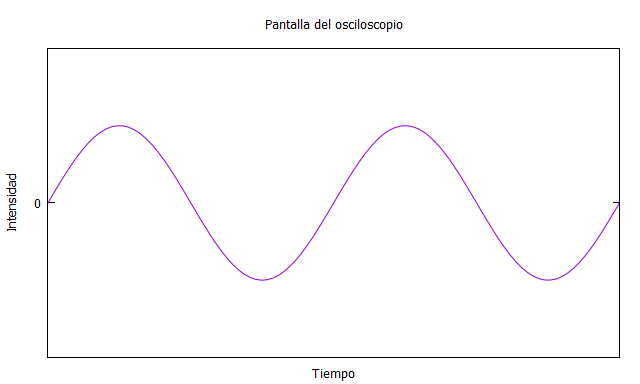
\includegraphics[width=10cm]{P10Sinusoide.png}
\caption{Esquema de la señal vista en el osciloscopio al aumentar el voltaje más allá del voltaje de frenado.}
\label{P10sinusoide}
\end{center}
\end{figure}
\begin{figure}[!ht]
\begin{center}
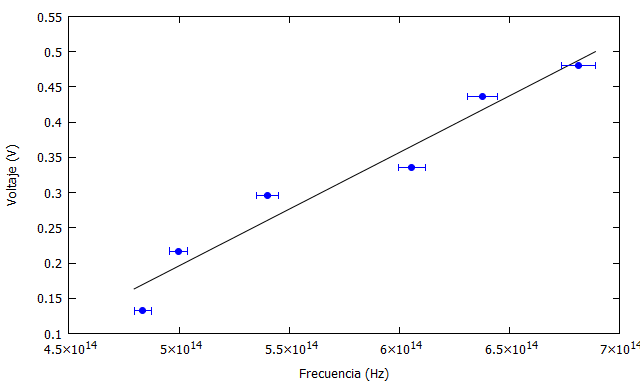
\includegraphics[width=10cm]{P10Anodotapado.png}
\caption{Representación del voltaje entre las placas en función de la frecuencia de la radiación con el ánodo tapado. Se incluye la recta de regresión lineal de pendiente $\unit[(1.61\pm0.19)\cdot10^{-15}]{V/Hz}$ y de ordenada en el origen $\unit[(-0.61\pm0.11)]{V}$. El coeficiente de correlación es $0.949$.}
\label{P10anodotapado}
\end{center}
\end{figure}

En la figura \ref{P10anodotapado} se ven los voltajes de frenado con el ánodo tapado. Efectivamente son distintos, lo cual indica que antes algunos electrones iban del ánodo al cátodo. En estas nuevas circunstancias el coeficiente de correlación lineal ha ascendido y es muy cercano a $1$, lo cual indica que los puntos se ajustan mejor a una recta y que los resultados experimentales son mejores. Esto es causado por haber eliminado una fuente de error: la señal que generaban los electrones que viajaban del ánodo al cátodo ---los cuales no se han tenido en cuenta al deducir la expresión (\ref{P10ecuacion})---.

La función de trabajo es $\unit[(9.7\pm1.7)\cdot10^{-20}]{J}$ y la constante de Planck obtenida experimentalmente en este caso es $\unit[(2.58\pm0.30)\cdot10^{-34}]{J\cdot s}$, con una discrepancia del $61\%$. Estos resultados son sorprendentes porque, a pesar de ajustarse mejor a una recta ---como se esperaba al eliminar el error producido por los electrones que viajan al revés---, la constante de Planck calculada tiene más discrepancia que en el caso anterior.

\subsection{Conclusiones}
Con esta práctica se ha podido comprobar el carácter corpuscular de la luz. Este se manifiesta cuando la luz es absorbida y emitida por los átomos. Es solo con el modelo corpuscular que se pueden explicar las observaciones realizadas; con el modelo ondulatorio las predicciones son completamente distintas.

La teoría clásica de la luz con un comportamiento ondulatorio es útil para explicar su propagación, pues fenómenos como el de difracción son claramente característicos de una onda. Sin embargo, para entender cómo es absorbida y emitida es necesario considerarla constituida por partículas ---que son llamadas fotones---.

Gracias a este modelo y con las medidas pertinentes se ha conseguido dar una aproximación de la constante de Planck.

Lo que propuso Einstein era rompedor con la física clásica y con todo lo que se creía saber sobre la luz. Y sin embargo se ha comprobado en esta práctica que funciona, lo cual nos dice que es fructífero proponer nuevas ideas revolucionarias para explicar fenómenos hasta el momento inexplicables.

\newpage
\section{Apéndice}
\subsection{Práctica 2. Reflexión y refracción en dioptrios planos}
La incertidumbre $u_2$ de la diferencia entre dos medidas de igual incertidumbre $u_1$ es
\begin{equation}\label{P2incdif}
u_2^2=\sqrt{u_1^2+u_1^2}=sqrt{2u_1^2}=\sqrt{2}u_1.
\end{equation}

Cuando se tienen diversas medidas de una misma magnitud, la incertidumbre estadística de la media es 
\begin{equation}\label{P2incmedia}
u_est^2=\frac{1}{n(n-1)}\sum_{i=1}^n(x_i-\bar{x}^2
\end{equation}

\end{document}